% =============================================================================
%  La escala importa — NO2 de fondo en España
%  Formato expositivo del REPORTE (figura -> descripción -> interpretación),
%  resultados del análisis completo y notación del curso de Estadística
%  Espacial (Dr. E. A. Chacón, UNI).
%
%  Compilar con pdfLaTeX. Las figuras se buscan en varias rutas: funciona
%  tanto en local (paper/ + ../output/figuras/) como en Overleaf con las
%  imágenes en figuras/ o sueltas junto al .tex.
% =============================================================================
\documentclass[11pt,a4paper]{article}

\usepackage[utf8]{inputenc}
\usepackage[T1]{fontenc}
\usepackage[spanish,es-noquoting]{babel}
\usepackage{lmodern}
\usepackage[margin=2.5cm]{geometry}
\usepackage{amsmath,amssymb,bm}
\usepackage{graphicx}
\graphicspath{{../output/figuras/}{output/figuras/}{figuras/}{./}}
\usepackage{booktabs}
\usepackage{longtable}
\usepackage{array}
\usepackage{caption}
\usepackage[table]{xcolor}
\usepackage{siunitx}
\usepackage[version=4]{mhchem}
\usepackage{enumitem}
\usepackage{titlesec}
\usepackage[hidelinks]{hyperref}

\sisetup{output-decimal-marker={,}, group-separator={\,}}

\definecolor{azul}{RGB}{28,72,122}
\definecolor{grisc}{RGB}{240,242,245}

% --- Encabezados en versalitas altas, al estilo del reporte ------------------
\titleformat{\section}{\normalfont\large\bfseries\color{azul}}{}{0pt}{\MakeUppercase}
\titleformat{\subsection}{\normalfont\normalsize\bfseries}{\thesubsection}{0.6em}{}
\titlespacing*{\section}{0pt}{16pt}{8pt}

% --- Rótulo de figura/tabla al estilo del reporte ----------------------------
\newcommand{\rotulo}[2]{%
  \vspace{4pt}\noindent\textbf{#1}\\[2pt]\emph{#2}\\[4pt]}

% =============================================================================
%  NOTACIÓN DEL CURSO
%  Localizaciones s, desplazamiento d (no h), proceso latente W y observable Y,
%  adyacencia A (la letra W está ocupada por el proceso).
% =============================================================================
\newcommand{\dom}{D}
\newcommand{\loc}{\bm{s}}
\newcommand{\loci}[1]{\bm{s}_{#1}}
\newcommand{\dvec}{\vec{d}}
\newcommand{\dsc}{d}
\newcommand{\Wp}[1]{W(#1)}
\newcommand{\Yp}[1]{Y(#1)}
\newcommand{\varesp}{\sigma^{2}}
\newcommand{\pepita}{\tau^{2}}
\newcommand{\escala}{\phi}
\newcommand{\suave}{\nu}
\newcommand{\corr}{\rho}
\newcommand{\Rphi}{\bm{R}_{\escala}}
\newcommand{\rangop}{r^{*}}
\newcommand{\Adj}{\bm{A}}
\newcommand{\Prec}{\bm{Q}}
\newcommand{\Esp}{\mathrm{E}}
\newcommand{\Var}{\mathrm{V}}
\newcommand{\Cor}{\mathrm{Cor}}
\newcommand{\Normal}{\mathcal{N}}
\newcommand{\Vg}{\mathcal{V}\!g}

\begin{document}

% =============================================================================
\begin{center}
{\Large\bfseries\color{azul} La escala importa: convergencia entre el
agrupamiento de fuentes industriales y su influencia sobre el \ce{NO2} de
fondo en España\par}

\vspace{8pt}
{\normalsize Randy Fernández Palomino \quad\textperiodcentered\quad
José Carhuaricra Cusipuma\par}
\vspace{3pt}
{\small\texttt{randy.fernandez.p@uni.pe} \quad\textperiodcentered\quad
\texttt{jose.carhuaricra@unh.edu.pe}\par}
\vspace{3pt}
{\small Estadística Espacial \quad\textperiodcentered\quad Doctorado en
Ciencias e Ingeniería Estadística\par}
{\small Universidad Nacional de Ingeniería (UNI) \quad\textperiodcentered\quad
2026\par}
\end{center}

\vspace{6pt}

% =============================================================================
\section{Resumen}

La atribución del \ce{NO2} de fondo a fuentes industriales o a urbanización
está mal condicionada en la mayoría de los países europeos porque ambos
factores son espacialmente colineales. España constituye una excepción: sus
grandes focos industriales están desacoplados de los focos urbanos. Este
trabajo explota esa separación aplicando las \textbf{tres ramas de la
estadística espacial} sobre el mismo contaminante, el mismo año y el mismo
dominio, y articulándolas en una cuarta pregunta que ninguna responde sola:
¿a qué escala espacial opera la influencia industrial?

La rama continua modela el campo de fondo sobre \num{212} estaciones y estima
un rango práctico de \SI{71}{\kilo\metre}, que cae a \SI{24}{\kilo\metre} tras
retirar la deriva; el kriging con deriva externa mejora el error del kriging
ordinario en un \SI{34.3}{\percent}. La rama discreta agrega a las \num{50}
provincias y encuentra que el efecto industrial desaparece: resiste cuatro
intentos de refutación y solo resulta significativo en el \SI{2.5}{\percent} de
\num{1000} zonificaciones alternativas. La rama puntual, que \emph{no observa
ninguna concentración}, ajusta un proceso agregado a las coordenadas de
\num{297} instalaciones E-PRTR y estima un diámetro efectivo del distrito
industrial de \SI{10.7}{\kilo\metre}. Un barrido independiente de anchos de
banda que acopla emisión y concentración sitúa la escala óptima de influencia
en \SI{10.0}{\kilo\metre} ($F = \num{13.86}$, $p = \num{2.5e-4}$); la razón
entre ambas estimaciones es \num{0.93}.

La desaparición del efecto a escala provincial no es falta de potencia sino un
efecto de la unidad de análisis: un radio de influencia de \SI{10}{\kilo\metre}
cubre el \SI{0.8}{\percent} de la provincia media española. Se deriva una cota
superior para el efecto industrial areal de \SI{0.956}{\micro\gram\per\cubic\metre},
el \SI{22.3}{\percent} de la media nacional de fondo.

\vspace{4pt}
\noindent\textbf{Palabras clave:} variación espacial continua, variación
espacial discreta, procesos puntuales, semivariograma, \textsc{maup}, cambio de
soporte, calidad del aire, \ce{NO2}.

% =============================================================================
\section{Introducción}

El dióxido de nitrógeno es, entre los contaminantes regulados, aquel en que la
pregunta «¿industria o tráfico?» permanece genuinamente abierta a escala
regional. A diferencia del material particulado, dominado por fuentes difusas y
transporte de largo alcance, el \ce{NO2} tiene una firma doble: emisiones
puntuales de gran magnitud procedentes de instalaciones industriales de
combustión, y emisiones lineales difusas asociadas al tráfico rodado.

Los modelos empíricos de calidad del aire de referencia —regresión de uso del
suelo y sus variantes de aprendizaje automático (Beelen et al., 2013; Chen et
al., 2019)— alcanzan capacidades predictivas notables pero no separan
mecanismos: sus covariables capturan simultáneamente urbanización, industria y
transporte porque en la mayoría del territorio europeo estos coinciden
espacialmente. El problema es de identificabilidad, no de método.

La geografía industrial española presenta una propiedad inusual: sus mayores
emisores de \ce{NOx} —Huelva, Tarragona, Puertollano, As Pontes, Avilés,
Algeciras— se localizan lejos de los grandes focos urbanos de Madrid y
Barcelona. Esa separación abre la posibilidad de estimar el efecto industrial
sin confundirlo con la urbanización.

\subsection*{Marco teórico: las tres ramas}

La estadística espacial se organiza en tres ramas según el \textbf{conjunto
índice} del proceso estocástico subyacente, y las tres se aplican aquí sobre el
mismo fenómeno:

\begin{table}[h]
\centering
\small
\begin{tabular}{@{}p{3.6cm}p{5.4cm}p{5.4cm}@{}}
\toprule
\textbf{Rama} & \textbf{Conjunto índice} & \textbf{Objeto observado} \\
\midrule
Variación espacial continua &
$\{\Wp{\loc} : \loc \in \dom \subset \mathbb{R}^2\}$, índice continuo &
$\Yp{\loci{i}}$ en localizaciones \textbf{no aleatorias} \\
\addlinespace
Variación espacial discreta &
$\dom = \{R_1,\dots,R_{50}\}$, índice discreto &
$\Yp{R_i}$ agregado sobre regiones \\
\addlinespace
Procesos puntuales &
el índice \textbf{es} la aleatoriedad &
el conjunto de localizaciones $\{\loci{i}\}$ \\
\bottomrule
\end{tabular}
\end{table}

\subsection*{Objetivos}

El \textbf{objetivo general} es estimar la escala espacial a la que opera la
influencia industrial sobre el \ce{NO2} de fondo en España, integrando las tres
ramas de la estadística espacial sobre un mismo territorio y contaminante. Los
objetivos específicos son:

\begin{enumerate}[label=\alph*), leftmargin=1.4em, itemsep=2pt]
  \item Caracterizar la variación espacial continua del \ce{NO2} de fondo
  mediante el semivariograma y la predicción espacial, separando la variación
  explicada por covariables de la no explicada.
  \item Analizar la variación espacial discreta agregando el contaminante a las
  \num{50} provincias (\textsc{nuts}-3) y modelándolo frente a densidad
  poblacional, emisiones y área, documentando los dos componentes del
  \textsc{maup}.
  \item Estimar el patrón espacial de las fuentes industriales del registro
  E-PRTR mediante un modelo de intensidad de proceso puntual y caracterizar su
  agregación de segundo orden.
  \item Contrastar dos estimaciones metodológicamente independientes de la
  escala de influencia y sintetizar las fortalezas y limitaciones de cada rama.
\end{enumerate}

\subsection*{Contribución}

Este trabajo no propone un estimador nuevo. Propone un \textbf{diseño de
contraste}: estimar la escala espacial de la influencia industrial por dos vías
metodológicamente independientes y comprobar si convergen. La primera vía
observa solo dónde están las instalaciones y no mira ninguna concentración; la
segunda observa concentraciones y pregunta a qué distancia deja de notarse la
emisión. No existe razón aritmética para que coincidan.

% =============================================================================
\section{Datos}

El dominio es la España peninsular más el archipiélago balear,
\SI{498522}{\kilo\metre\squared}, en \textsc{epsg}:3035 (proyección
equiareal). Se excluyen Canarias, Ceuta y Melilla porque las tres ramas
presuponen un dominio conexo. Esta exclusión tiene una consecuencia que se
declara por adelantado: \textbf{Canarias concentra el \SI{24}{\percent} del
\ce{NOx} industrial español} en siete centrales diésel.

\rotulo{Tabla 1}{Fuentes de datos y trazabilidad}

\begin{center}
\small
\begin{tabular}{@{}p{3.4cm}p{2.2cm}p{4.4cm}p{4.2cm}@{}}
\toprule
\textbf{Variable} & \textbf{Fuente} & \textbf{Servicio} & \textbf{Función} \\
\midrule
Geometrías \textsc{nuts} 2021 & EEA &
\texttt{NUTS\_RG\_01M\_2021\_3035} & Soporte areal, \num{50} provincias \\
\ce{NO2} por estación (2023) & EEA &
\texttt{ParquetFile}, dataset E1a & Variable respuesta continua \\
Clasificación de estaciones & EEA &
\texttt{DiscoData AirQualityStatistics} & Separar fondo de tráfico \\
Instalaciones IED & EEA &
\texttt{Air/IED\_SiteMap/MapServer} & Patrón puntual \\
Emisiones \ce{NOx} (E-PRTR) & EEA &
\texttt{DiscoData [IED].[v1r2]} & Marcas del patrón \\
\ce{NO2} troposférico & Copernicus &
\texttt{openEO, SENTINEL\_5P\_L2} & Covariable satelital \\
Cobertura del suelo & Copernicus &
\texttt{CORINE CLC2018}, \SI{100}{\metre} & Covariables $Z_j(\loc)$ \\
Densidad de población & Eurostat &
\texttt{demo\_r\_d3dens} & Covariable areal \\
\bottomrule
\end{tabular}
\end{center}

\subsection*{Tres decisiones que condicionan todo lo demás}

\textbf{Solo estaciones de fondo alimentan el modelo geoestadístico.} De las
\num{462} estaciones dentro del dominio, \num{212} están clasificadas como
\emph{background} y \num{250} como industriales o de tráfico. Las de tráfico
miden a microescala: el \ce{NO2} decae entre el \SI{60}{\percent} y el
\SI{80}{\percent} en los primeros \SI{50}{\metre} desde la calzada. En la
notación del modelo, una estación de tráfico no observa $\Wp{\loc}+\varepsilon$
con $\varepsilon$ de media nula, sino $\Wp{\loc} + \text{recargo}(\loc) +
\varepsilon$: no es ruido, es otro proceso. Excluirlas no es una pérdida sino un
cambio de papel — se reservan como validación externa.

\textbf{Desagrupamiento por celdas de \SI{25}{\kilo\metre}.} La red de medición
está sesgada hacia zonas urbanas. Sin corregir, la media muestral es
\SI{11.36}{\micro\gram\per\cubic\metre}; tras desagrupar,
\SI{8.58}{\micro\gram\per\cubic\metre}. Como del campo existe \textbf{una sola
realización}, la estacionariedad y la isotropía no se contrastan: se suponen, y
el desagrupamiento evita que el diseño de muestreo se confunda con la media del
proceso.

\textbf{Normalización costera de CORINE.} En el ráster CLC2018 el mar es la
clase 523, no \emph{nodata}. Sin corregirlo, provincias costeras como Cádiz
aparecen con fracción artificial \num{0.15} cuando el valor correcto sobre
tierra es \num{0.72}.

% =============================================================================
\section{Metodología}

\rotulo{Tabla 2}{Etapas metodológicas}

\begin{center}
\small
\begin{tabular}{@{}p{0.9cm}p{3.2cm}p{5.4cm}p{4.6cm}@{}}
\toprule
\textbf{Paso} & \textbf{Módulo} & \textbf{Descripción técnica} &
\textbf{Resultado} \\
\midrule
1 & Ingesta y depuración &
Lectura del Parquet de la EEA, filtrado al dominio, unificación a
\textsc{epsg}:3035, desagrupamiento a \SI{25}{\kilo\metre}, deduplicación del
patrón puntual por \texttt{InspireSiteId}. &
Conjunto armonizado en metros reales. \\
\addlinespace
2 & Variación continua &
Semivariograma empírico sobre la respuesta y sobre los residuos de la deriva;
ajuste del modelo de correlación; predicción por kriging con deriva externa
frente a kriging ordinario. &
Superficie predicha en rejilla de \SI{2}{\kilo\metre} y mapa de error. \\
\addlinespace
3 & Variación discreta &
Agregación a \num{50} provincias, grafo de vecindad, $I$ de Moran y \textsc{lisa},
contrastes robustos del multiplicador de Lagrange y \textsc{sar} con regresión.
La misma especificación se repite sobre las \num{16} comunidades autónomas
(componente de escala) y sobre \num{1000} particiones alternativas en
\num{16} grupos por $k$-medias (componente de zonificación). &
Modelo areal, cota del efecto y diagnóstico \textsc{maup} completo. \\
\addlinespace
4 & Procesos puntuales &
Contraste de cuadrantes por Monte Carlo, modelo de intensidad con covariables
CORINE, función $K$ inhomogénea con envolventes y ajuste de un proceso
agregado. &
Intensidad $\lambda(\loc)$ y escala de agregación. \\
\addlinespace
5 & Síntesis &
Barrido de anchos de banda de la superficie de presión de emisión y contraste
$F$ anidado contra el modelo de la etapa 2. &
Escala de influencia y contraste de convergencia. \\
\bottomrule
\end{tabular}
\end{center}

% =============================================================================
\section{Modelos}

\subsection*{1. Variación espacial continua: semivariograma y predicción}

El campo de fondo se modela como un proceso latente gaussiano estacionario e
isótropo más error de medición:

\begin{equation}
\Yp{\loci{i}} \;=\; \underbrace{\bm{x}^{\!\top}\!(\loci{i})\bm{\beta}}
_{\text{variación espacial explicada}}
\;+\; \underbrace{\Wp{\loci{i}}}_{\text{no explicada}}
\;+\; \varepsilon_i,
\qquad \varepsilon_i \overset{iid}{\sim} \Normal(0,\pepita)
\end{equation}

con $\{\Wp{\loc}\}$ un proceso gaussiano estacionario e isótropo de varianza
$\varesp$ y función de correlación $\corr_{\escala}(\dsc)$, donde $\dsc$ es la
distancia entre localizaciones. En forma matricial,
$\bm{Y}\sim\Normal_n(\bm{X}\bm{\beta},\, \varesp\Rphi + \pepita\bm{I}_n)$.

El \textbf{semivariograma teórico} y su relación con la correlación son

\begin{equation}
\Vg(\loci{i},\loci{j}) = \tfrac{1}{2}\Var\!\big[\Wp{\loci{i}}-\Wp{\loci{j}}\big]
= \varesp\big(1-\Cor[\Wp{\loci{i}},\Wp{\loci{j}}]\big),
\end{equation}

de donde, para el proceso \emph{observado} con error de medición,
$\Vg_Y(\dsc) = \varesp(1-\corr(\dsc)) + \pepita$: \textbf{la pepita es
$\pepita$}, la variación no espacial. Si además hay tendencia, el
semivariograma incorpora un término cuadrático en la distancia, razón por la
cual el rango se estima sobre residuos y no sobre la variable bruta. El
estimador empleado es

\begin{equation}
\widehat{\Vg}_{Y}(\dsc) \;=\; \frac{1}{2n_{ij}}
\sum_{i,j\,:\,\lVert \loci{i}-\loci{j}\rVert = \dsc \pm \epsilon}
(y_i-y_j)^2 ,
\end{equation}

con $n_{ij}$ el número de pares en la banda $\dsc\pm\epsilon$. El
\textbf{rango práctico} se define como la distancia $\rangop$ tal que
$\corr(\rangop) = \num{0.05}$.

La \textbf{predicción} es la distribución condicional de una normal
multivariante. Conviene distinguir dos objetivos que comparten media pero no
varianza:

\begin{align}
\bm{\mu}_{y^*\mid y} &= \bm{X}^{*}\bm{\beta}
+ \bm{\Sigma}_{w^*\!,w}\big(\bm{\Sigma}_w+\pepita\bm{I}\big)^{-1}
(\bm{y}-\bm{X}\bm{\beta}) \\[2pt]
\bm{\Sigma}_{y^*\mid y} &= \pepita\bm{I} \;+\;
\bm{\Sigma}_{w^*} - \bm{\Sigma}_{w^*\!,w}
\big(\bm{\Sigma}_w+\pepita\bm{I}\big)^{-1}\bm{\Sigma}_{w,w^*}
\end{align}

Predecir el \emph{campo latente} $\Wp{\loc^{*}}$ en un sitio nuevo no es lo
mismo que predecir una \emph{observación nueva} $\Yp{\loc^{*}}$: la diferencia
es exactamente $\pepita\bm{I}$. El predictor $\bm{\mu}_{w^*\mid y}$ es lo que
la literatura geoestadística denomina \emph{kriging}.

\subsection*{2. Variación espacial discreta: grafo, Moran y \textsc{sar}}

Sobre las $n=\num{50}$ provincias se define el vecindario de primer orden
$\mathcal{N}_i$ y la \textbf{matriz de adyacencia} $\Adj$, con $A_{ij}=1$ si
$R_j\in\mathcal{N}_i$. La estructura resultante es un grafo no dirigido
$\mathcal{G}=(V,E)$. El diagnóstico de asociación espacial emplea

\begin{equation}
I=\frac{n\sum_i\sum_j a_{ij}(Y_i-\bar{Y})(Y_j-\bar{Y})}
       {\big(\sum_{i\neq j}a_{ij}\big)\sum_i (Y_i-\bar{Y})^2},
\qquad
\Esp[I] = -\frac{1}{n-1} \;=\; \num{-0.020}.
\end{equation}

El modelo areal se especifica como un \textbf{\textsc{sar} con regresión}
—conocido en la literatura econométrica como modelo de error espacial— en el
que el autorregresivo se impone sobre el residuo
$\bm{U}=\bm{Y}-\bm{X}\bm{\beta}$:

\begin{equation}
\bm{U}=\bm{B}\bm{U}+\bm{\varepsilon}
\quad\Longrightarrow\quad
\bm{Y} = \bm{B}\bm{Y} + (\bm{I}-\bm{B})\bm{X}\bm{\beta} + \bm{\varepsilon},
\qquad \bm{B}=\alpha\,\bm{D}_a^{-1}\Adj,
\end{equation}

con la especificación propia si $|\alpha|<1$. La respuesta es
$y_i = \beta_0 + \beta_1\log d_i + \beta_2\log(1+m_i) + \beta_3\log a_i + u_i$,
donde $d_i$ es la densidad de población, $m_i$ las emisiones totales y $a_i$ el
área.

La \textbf{media areal de bloque} $y_i$ se calcula promediando la superficie
predicha \textbf{en escala cruda} sobre cada polígono. Como la rama continua
modela $\log \Yp{\loc}$, esto exige deshacer la transformación antes de
promediar:
\[
y_i \;=\; \frac{1}{|R_i|}\int_{R_i} \exp\!\big(\hat{\Yp{\loc}}\big)\,d\loc ,
\]
y \emph{no} volver a transformar después. El orden importa: promediar en escala
logarítmica daría la media geométrica de las concentraciones, que subestima
sistemáticamente la media aritmética por la desigualdad de Jensen, y no es la
magnitud sobre la que se legisla. La inclusión conjunta de $\log m_i$ y $\log a_i$ resuelve el desajuste
dimensional entre una respuesta intensiva y un predictor extensivo: equivale a
modelar $\log(m/a^{\theta})$ con $\theta=-\beta_3/\beta_2$, de modo que no se
impone \emph{a priori} si la industria actúa como masa total o como densidad.

\subsection*{3. Procesos puntuales: intensidad y segundo orden}

El conjunto de instalaciones se modela como un proceso puntual sobre el
dominio. Su distribución se caracteriza mediante la medida de conteo $N(A)$, y
se exige la propiedad de proceso \textbf{ordenado} —no puede haber eventos
coincidentes múltiples—, que es lo que justifica la deduplicación por
\texttt{InspireSiteId}. El modelo de intensidad es

\begin{equation}
\log \lambda(\loc) \;=\; B(\loc) + \theta_1 Z_1(\loc) + \cdots +
\theta_p Z_p(\loc),
\end{equation}

donde los predictores $Z_j(\loc)$ \textbf{deben conocerse en todo el dominio},
no solo en los eventos: de ahí que sean rásteres CORINE y no atributos de
planta. La verosimilitud es
$L(\theta)\propto \exp\{-\int_\dom \lambda_\theta(\loc)\,d\loc\}
\prod_i \lambda_\theta(\loci{i})$.

Las propiedades de segundo orden se resumen en la correlación por pares y en la
función $K$:

\begin{equation}
g_2(\loc,\loc') = \frac{\lambda_2(\loc,\loc')}{\lambda(\loc)\lambda(\loc')}
\overset{\text{independencia}}{=} 1,
\qquad
K(t) = \lambda^{-1}\,\Esp[N_0(t)]
\overset{\text{Poisson homog.}}{=} \pi t^2 .
\end{equation}

La agregación residual se modela con un \textbf{proceso agregado}: padres de un
Poisson de intensidad $\kappa$, descendencia dispersada en torno a cada padre,
y lo observado son los hijos. Con dispersión gaussiana de desviación típica
$\sigma$, el diámetro efectivo del conglomerado es $4\sigma$, que contiene
aproximadamente el \SI{95}{\percent} de la dispersión.

\subsection*{4. Síntesis: la superficie de presión de emisión}

Se construye una superficie ponderando cada instalación por el logaritmo de su
masa de \ce{NOx} y suavizando con un núcleo gaussiano de ancho de banda $h$:

\begin{equation}
P_h(\loc) \;=\; \sum_{i=1}^{n} \log(1+m_i)\,
\kappa_h\!\left(\lVert\loc-\loci{i}\rVert\right).
\end{equation}

Para cada $h\in\{5,10,15,25,40,60,100\}$ km se añade $\log P_h$ al modelo de la
ecuación (1) y se comparan por error de validación cruzada y contraste $F$
anidado. El $h$ óptimo es \textbf{una estimación, no una elección de diseño};
esta es la diferencia con la práctica habitual de fijar radios de influencia a
priori. El uso de $\log(1+m_i)$ y no de $m_i$ responde a la asimetría de las
marcas (coeficiente \num{3.30}): las diez mayores instalaciones concentran el
\SI{17.2}{\percent} del \ce{NOx} total y dominarían la superficie sin
transformar.

\rotulo{Tabla 3}{Resumen de los modelos por rama}

\begin{center}
\small
\begin{tabular}{@{}p{2.5cm}p{3.3cm}p{3.4cm}p{5.0cm}@{}}
\toprule
\rowcolor{grisc}
\textbf{Rama} & \textbf{Modelo} & \textbf{Variable dependiente} &
\textbf{Estructura de covarianza} \\
\midrule
Continua & Modelo lineal espacial, kriging con deriva externa &
$\Yp{\loci{i}}$: \ce{NO2} de fondo (\si{\micro\gram\per\cubic\metre}) &
$\varesp\Rphi + \pepita\bm{I}$, construida con \textbf{distancias} \\
\addlinespace
Discreta & \textsc{sar} con regresión (error espacial) &
$\Yp{R_i}$: media areal por provincia &
$\Prec^{-1} + \varesp\bm{I}$, construida con un \textbf{grafo} \\
\addlinespace
Puntual & Modelo de intensidad y proceso agregado &
$N(A)$: conteo de instalaciones en $A$ &
Intensidad $\lambda(\loc)$ y función $K(t)$ \\
\bottomrule
\end{tabular}
\end{center}

\noindent Nótese que las dos primeras filas son \textbf{el mismo modelo}
$\Normal(\bm{X}\bm{\beta},\ \text{espacial}+\text{ruido})$: lo único que cambia
es si el efecto espacial se construye a partir de distancias o de un grafo. La
covarianza es densa e informa de la dependencia marginal; la precisión es
dispersa e informa de la independencia condicional.

% =============================================================================
\section{Resultados}

\subsection*{Objetivo a): la variación espacial continua}

\rotulo{Figura 1}{Distribución de la concentración de \ce{NO2} en las
estaciones de fondo}

\begin{center}
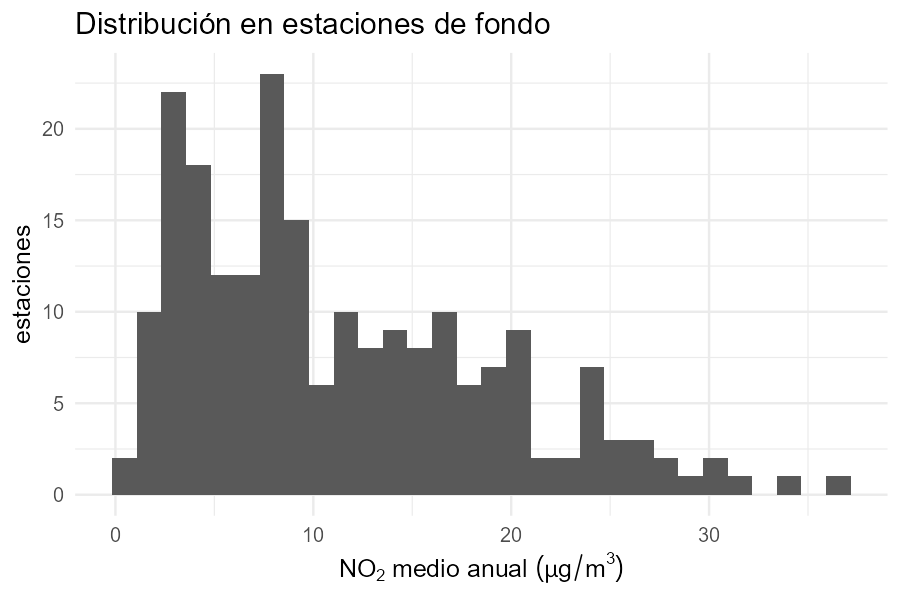
\includegraphics[width=0.66\textwidth]{01_histograma.png}
\end{center}

La distribución de las \num{212} estaciones de fondo es asimétrica a la
derecha, lo que motiva trabajar en escala logarítmica. La media desagrupada es
\SI{8.58}{\micro\gram\per\cubic\metre} frente a
\SI{11.36}{\micro\gram\per\cubic\metre} sin corregir: la diferencia de
\SI{2.78}{\micro\gram\per\cubic\metre} es enteramente atribuible al sesgo
urbano del diseño de la red, no al proceso.

\rotulo{Figura 2}{Semivariograma empírico y modelo ajustado}

\begin{center}
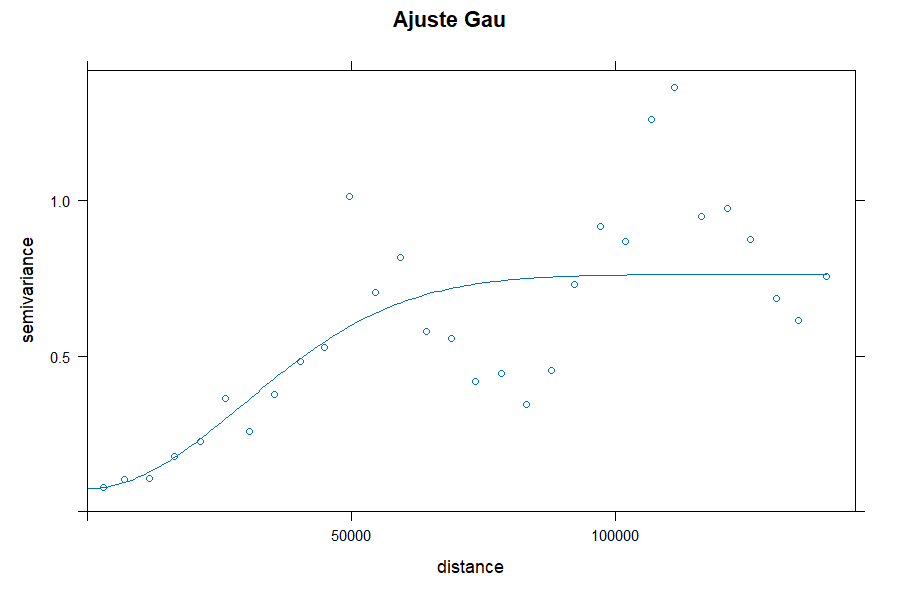
\includegraphics[width=0.62\textwidth]{04_variograma_ajustado.png}
\end{center}

El semivariograma empírico crece hasta estabilizarse en una meseta. El ajuste
proporciona un \textbf{rango práctico de \SI{71}{\kilo\metre}} en el sentido
$\corr(\rangop)=\num{0.05}$, y una \textbf{pepita relativa
$\pepita/(\varesp+\pepita)$ del \SI{9.6}{\percent}}. Este último número
responde directamente a una de las preguntas exploratorias del análisis
espacial —¿es la variación espacial más fuerte que la no espacial?—: el
\SI{90.4}{\percent} de la variabilidad está espacialmente estructurada.

Se declara una limitación del ajuste: el modelo seleccionado corresponde al
límite suave de la familia de Matérn (parámetro de suavizado $\suave$ grande) e
implica variación por debajo de la menor distancia entre estaciones, supuesto
poco creíble en calidad del aire. Se controla mediante el variograma residual.

\rotulo{Figura 3}{Semivariograma sobre la respuesta y sobre los residuos de la
deriva}

\begin{center}
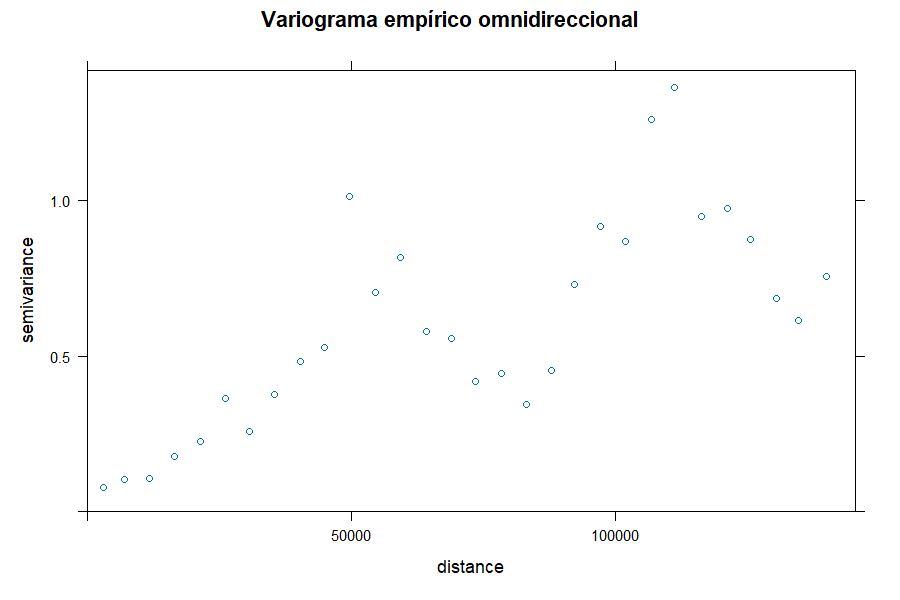
\includegraphics[width=0.48\textwidth]{02_variograma_omni.png}\hfill
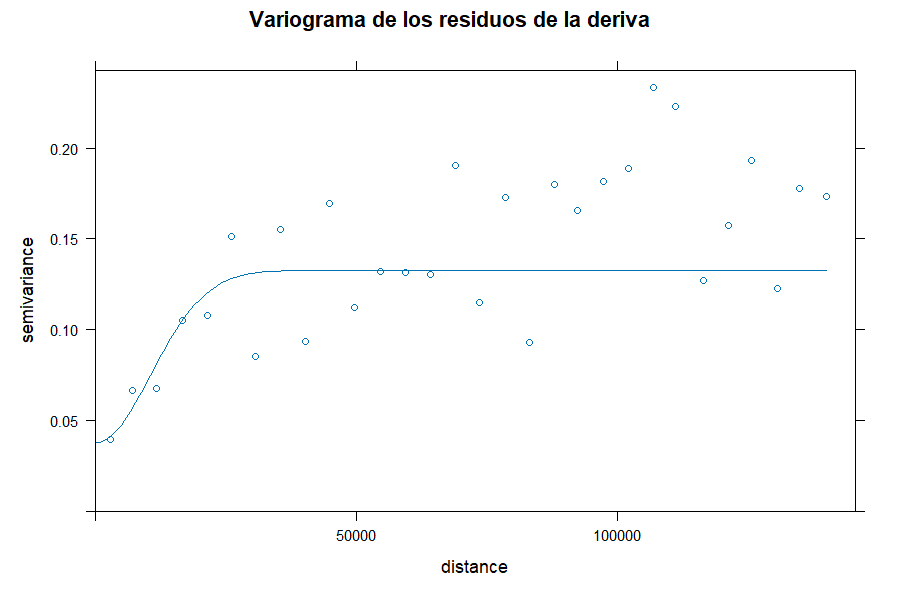
\includegraphics[width=0.48\textwidth]{05_variograma_residual.png}
\end{center}

La comparación es el resultado central de esta rama. Las covariables
—\ce{NO2} troposférico de Sentinel-5P, fracciones de uso del suelo a \SI{1}{}
y \SI{5}{\kilo\metre}, y altitud— \textbf{absorben el \SI{76}{\percent} de la
varianza}: la varianza pasa de \num{0.650} a \num{0.155} y el rango práctico de
\SI{71}{} a \textbf{\SI{24}{\kilo\metre}}.

La interpretación es directa en términos de la ecuación (1): el término
$\bm{x}^{\!\top}(\loc)\bm{\beta}$ recoge la variación espacial explicada y
$\Wp{\loc}$ la no explicada. Además, una tendencia infla el semivariograma con
un término cuadrático en la distancia, de modo que el rango de
\SI{71}{\kilo\metre} sobre la variable bruta \emph{sobreestima} la
dependencia espacial genuina; el valor interpretable es el residual.

\rotulo{Figura 4}{Predicción espacial: kriging ordinario frente a kriging con
deriva externa}

\begin{center}
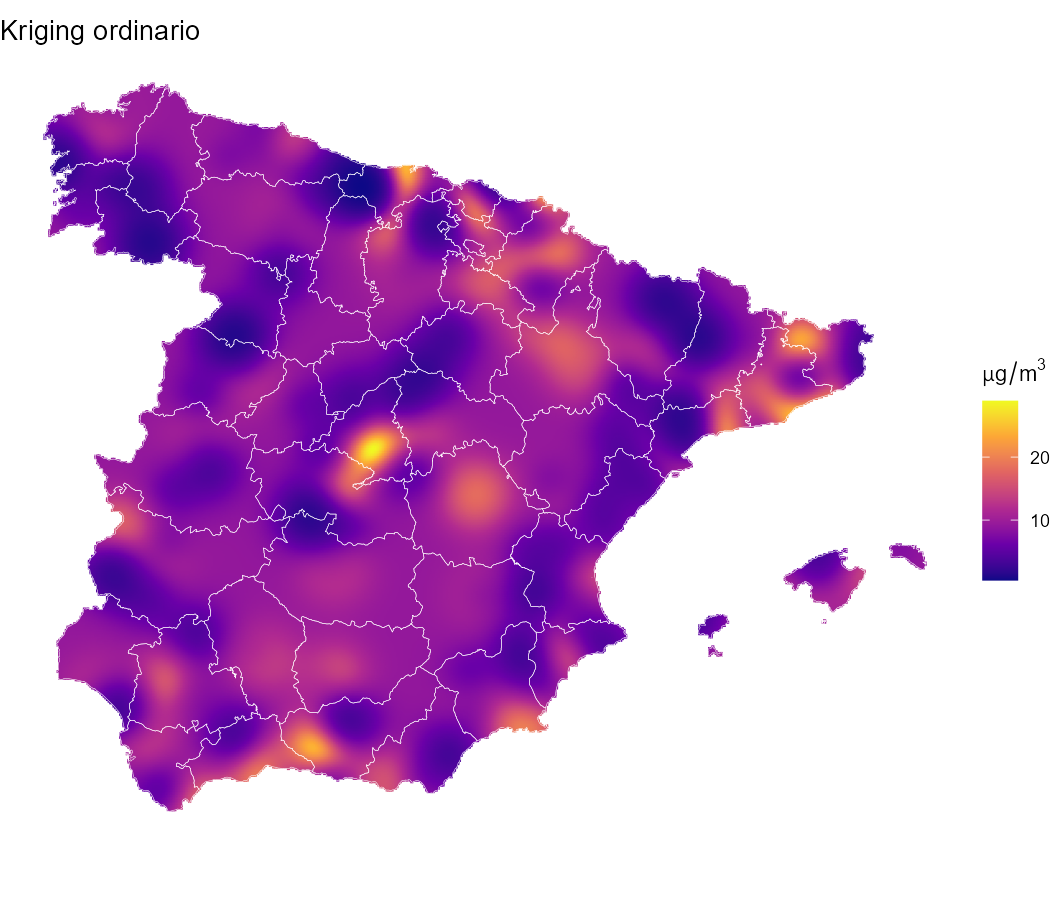
\includegraphics[width=0.48\textwidth]{06_mapa_ko.png}\hfill
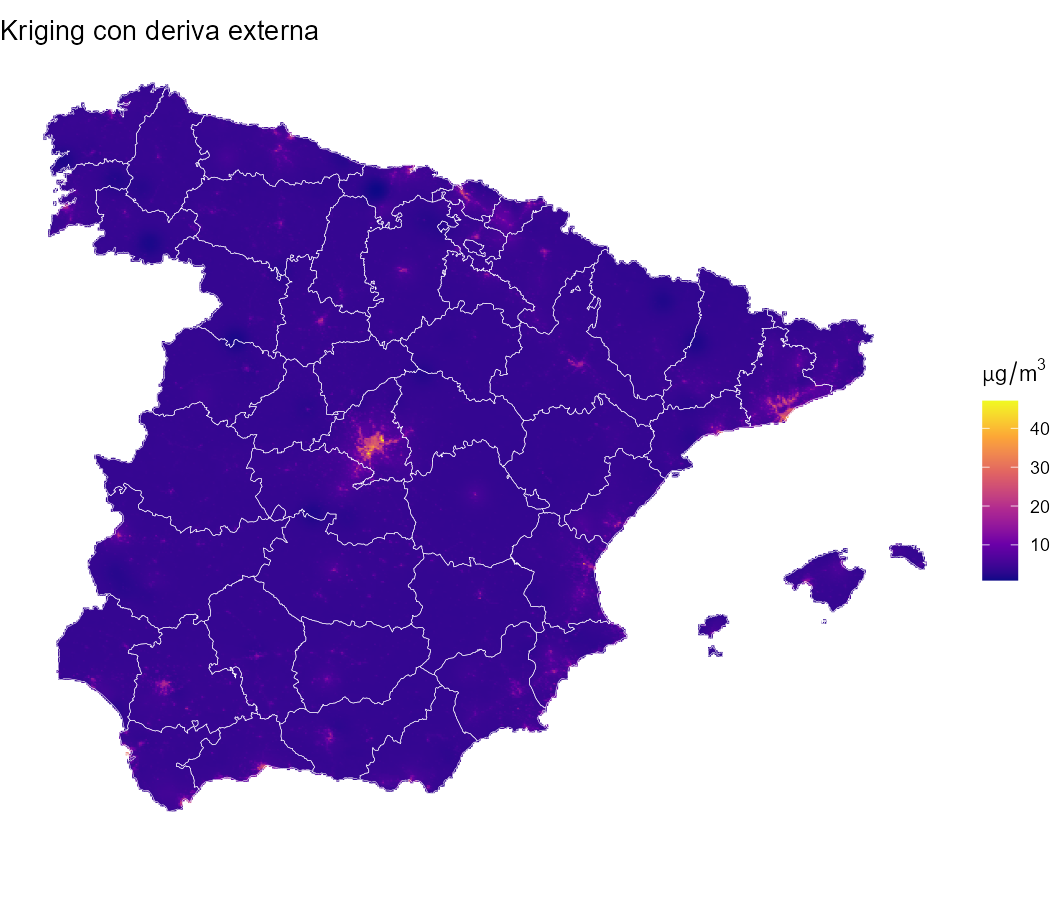
\includegraphics[width=0.48\textwidth]{07_mapa_kde.png}
\end{center}

\rotulo{Tabla 4}{Validación cruzada \emph{leave-one-out} sobre \num{212}
estaciones de fondo}

\begin{center}
\small
\begin{tabular}{@{}lccc@{}}
\toprule
 & \textbf{RMSE} & \textbf{$R^2$} & \textbf{Sesgo} \\
\midrule
Kriging ordinario & \num{5.565} & \num{0.481} & \num{0.933} \\
\rowcolor{grisc}
Kriging con deriva externa & \num{3.657} & \num{0.776} & \num{0.156} \\
Mejora & \SI{-34.3}{\percent} & --- & --- \\
\bottomrule
\end{tabular}
\end{center}

El kriging con deriva externa reduce el error en un \SI{34.3}{\percent} y
prácticamente elimina el sesgo. El mapa de la derecha muestra estructura fina
que el de la izquierda no puede reproducir, porque el kriging ordinario solo
dispone de la información de las propias estaciones.

La cobertura empírica del intervalo nominal al \SI{95}{\percent} es
\num{0.910}. Conviene precisar contra qué se valida: al comparar contra
observaciones de estaciones, el objetivo correcto es $\Yp{\loc^{*}}\mid\bm{Y}$
—que incluye $\pepita\bm{I}$— y no el campo latente
$\Wp{\loc^{*}}\mid\bm{Y}$. La ligera infracobertura debe leerse a la luz de esa
distinción.

\rotulo{Figura 5}{Error de predicción}

\begin{center}
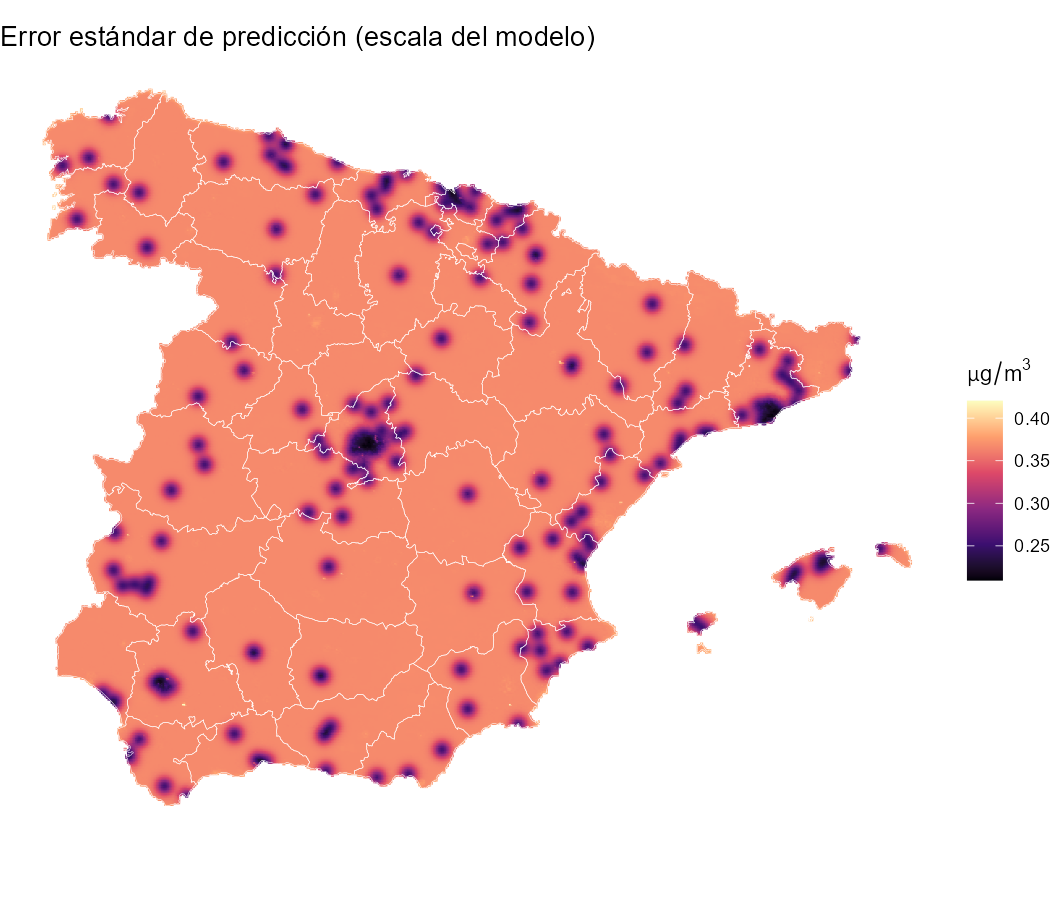
\includegraphics[width=0.60\textwidth]{08_mapa_error.png}
\end{center}

La incertidumbre no es uniforme: crece en las zonas de baja densidad de
estaciones, que es exactamente lo que la varianza de kriging debe reflejar. El
mapa señala dónde las conclusiones son más frágiles.

\subsection*{Validación externa: el recargo local}

El resultado más informativo de esta rama procede de las estaciones
\emph{excluidas} del ajuste. El sesgo del fondo predicho respecto a lo medido
es de \SIrange{2.9}{4.8}{\micro\gram\per\cubic\metre} en estaciones de tráfico
frente a \SIrange{0.5}{1.5}{\micro\gram\per\cubic\metre} en industriales. En
entorno rural las estaciones industriales miden un \SI{52}{\percent} más que
las de fondo (\num{5.95} frente a
\SI{3.91}{\micro\gram\per\cubic\metre}); en entorno urbano la diferencia se
anula.

\textbf{La industria eleva el \ce{NO2} donde el fondo es bajo, pero queda
sepultada por el tráfico en las ciudades.} Esto valida además la decisión de
excluir las estaciones de tráfico: el recargo medido cuantifica precisamente el
término que impide tratarlas como realizaciones del campo regional.

% -----------------------------------------------------------------------------
\subsection*{Objetivo b): la variación espacial discreta}

\rotulo{Figura 6}{Grafo de vecindad sobre las provincias}

\begin{center}
\includegraphics[width=0.86\textwidth]{44_grafo_vecindad.png}
\end{center}

Con contigüidad, el grafo $\mathcal{G}=(V,E)$ tiene \textbf{cuatro componentes
conexas}: península, Mallorca, Menorca y Eivissa--Formentera. Las islas quedan
sin vecinos con quien compartir información, y los contrastes de dependencia no
están definidos sobre un grafo disconexo. Con $k=5$ vecinos más próximos el
grafo se reconecta en una sola componente. Esta es la razón de usar
$k$-vecinos y no contigüidad en todo el diagnóstico areal.

\rotulo{Figura 7}{Diagrama de dispersión de Moran y agrupamientos locales}

\begin{center}
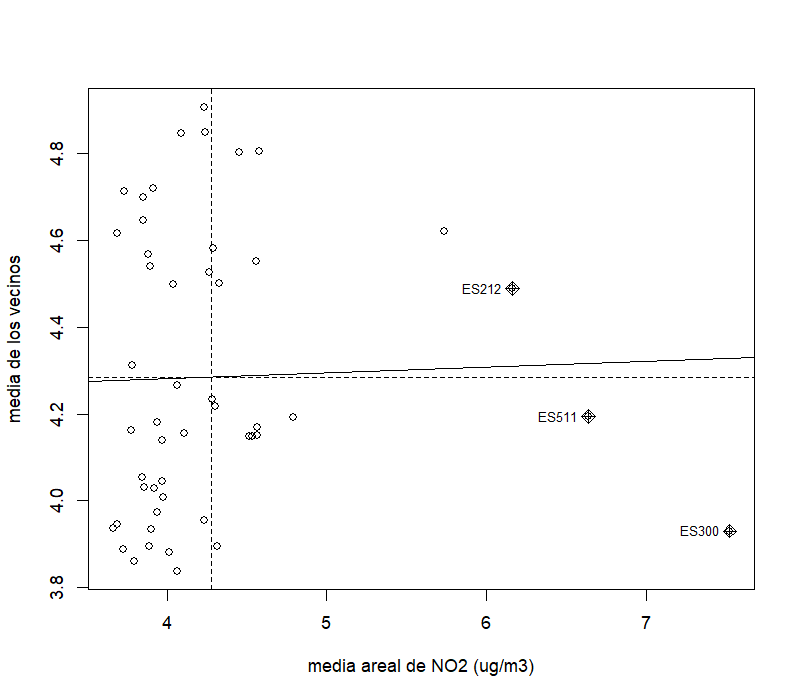
\includegraphics[width=0.48\textwidth]{40_moran_scatter.png}\hfill
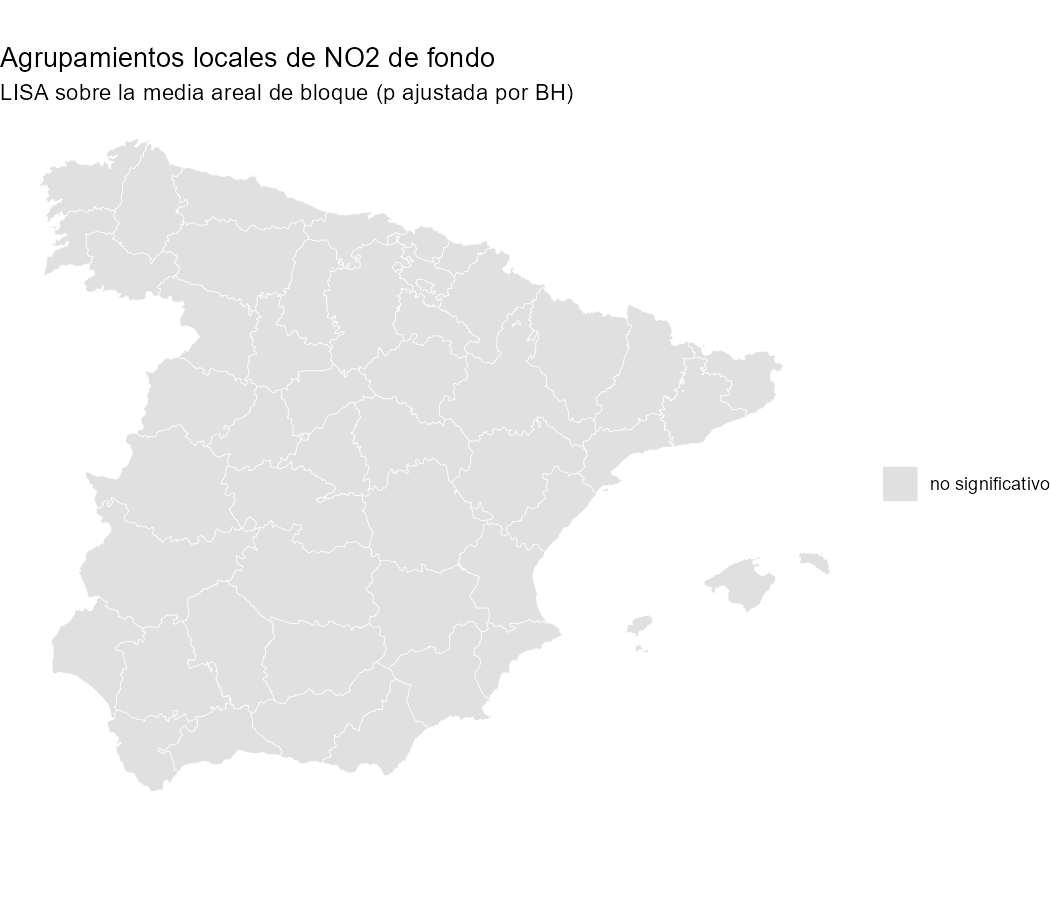
\includegraphics[width=0.48\textwidth]{41_lisa.png}
\end{center}

\rotulo{Tabla 5}{Asociación espacial global, $n=\num{50}$, $k=5$ vecinos}

\begin{center}
\small
\begin{tabular}{@{}lccc@{}}
\toprule
 & \textbf{$I$ de Moran} & \textbf{$\Esp[I]$ bajo $H_0$} & \textbf{$p$} \\
\midrule
Sobre la respuesta (media areal) & \num{0.013} & \num{-0.020} & \num{0.32} \\
\rowcolor{grisc}
Sobre los residuos del \textsc{mco} & \num{0.187} & \num{-0.020} &
\num{0.0019} \\
\bottomrule
\end{tabular}
\end{center}

El valor sobre la respuesta no es «cero» sino esencialmente su esperanza bajo
independencia, $\Esp[I]=-1/(n-1)=\num{-0.020}$. El hallazgo relevante es que
\textbf{la dependencia espacial aparece después de condicionar}, no antes: es
el caso inverso al ejemplo canónico de independencia condicional, donde
condicionar destruye la dependencia. Aquí condicionar en densidad y área la
crea, y eso es lo que justifica un modelo de error espacial y no un modelo de
contagio entre provincias.

Los contrastes robustos del multiplicador de Lagrange separan limpiamente hacia
el error espacial ($RS^{*}_{err}$: $p=\num{0.0015}$; $RS^{*}_{lag}$:
$p=\num{0.023}$). El \textsc{sar} con regresión ajustado da
$\hat\alpha=\num{0.446}$ ($p=\num{0.0090}$), \textbf{holgadamente dentro del
intervalo de propiedad $(-1,1)$}, y absorbe íntegramente la autocorrelación
($p=\num{0.54}$ sobre sus residuos).

\rotulo{Tabla 6}{Robustez del resultado nulo industrial}

\begin{center}
\small
\begin{tabular}{@{}lc@{}}
\toprule
\textbf{Especificación} & \textbf{$p$ de la industria} \\
\midrule
\textsc{mco}, emisiones totales & \num{0.63} \\
\textsc{mco}, presión a \SI{10}{\kilo\metre} & \num{0.36} \\
\textsc{mco} sin Madrid (Cook $=\num{0.97}$) & \num{0.90} \\
\textsc{sar} con regresión (error espacial) & \num{0.68} \\
\bottomrule
\end{tabular}
\end{center}

A escala provincial el coeficiente de las emisiones industriales no es
significativo ($\hat\beta_2=\num{-0.019}$, $p=\num{0.63}$), mientras que la
densidad de población lo es intensamente ($\hat\beta_1=\num{0.575}$,
$p=\num{2.1e-9}$). Los factores de inflación de la varianza son inferiores a
\num{1.8}, de modo que la colinealidad no explica el resultado. Ninguno de los
cuatro intentos de refutación lo revierte.

Los dos componentes del \textsc{maup} se documentan por separado.

\subsection*{Componente de escala: qué ocurre a \textsc{nuts}-2}

Al repetir la misma especificación sobre las \num{16} comunidades autónomas
aparece un coeficiente industrial \textbf{negativo y significativo}
($\hat\beta_2=\num{-0.548}$, $p=\num{0.0062}$), con un $R^2$ ajustado de
\num{0.776} frente al \num{0.601} de \textsc{nuts}-3. Tomado aisladamente, el
resultado diría que más emisión industrial implica menos \ce{NO2}, lo que
carece de sentido físico.

El diagnóstico de influyentes lo explica por completo. Madrid presenta una
distancia de Cook de \num{4.64}, \textbf{dieciocho veces el umbral $4/n$} y
diecisiete veces la siguiente observación. Es la única \textsc{nuts}-2 que
coincide prácticamente con una sola provincia, de modo que en un conjunto de
dieciséis unidades actúa como punto de apalancamiento y arrastra la regresión
por sí sola. Excluyéndola, el coeficiente cae a \num{-0.060}
($p=\num{0.69}$) y el $R^2$ ajustado a \num{0.602}, prácticamente idéntico al
provincial. \emph{La agregación infla el ajuste aparente sin aportar
información.}

\rotulo{Tabla 7}{Sensibilidad de especificación del efecto industrial a
\textsc{nuts}-2}

\begin{center}
\small
\begin{tabular}{@{}lccc@{}}
\toprule
\textbf{Especificación} & \textbf{Coef.} & \textbf{$p$} & \textbf{$R^2$ aj.} \\
\midrule
\textsc{nuts}-3, referencia ($n=\num{50}$) & \num{-0.0195} & \num{0.632} &
\num{0.601} \\
\midrule
\rowcolor{grisc}
\textsc{nuts}-2, misma especificación & \num{-0.5483} & \num{0.0062} &
\num{0.776} \\
\textsc{nuts}-2, sin el término de área & \num{-0.3328} & \num{0.065} &
\num{0.689} \\
\textsc{nuts}-2, conteo de instalaciones (log) & \num{-0.6784} & \num{0.028} &
\num{0.718} \\
\textsc{nuts}-2, conteo sin transformar & \num{-0.0403} & \num{0.010} &
\num{0.757} \\
\rowcolor{grisc}
\textsc{nuts}-2, excluyendo Madrid ($n=\num{15}$) & \num{-0.0604} &
\num{0.685} & \num{0.602} \\
\bottomrule
\end{tabular}
\end{center}

La tabla precisa dónde está la fragilidad. El efecto industrial a
\textsc{nuts}-2 \textbf{no es sensible a cómo se mida la industria}: sobrevive
al cambio de masa emitida a conteo de instalaciones, transformado o no. Lo que
lo hace desaparecer es retirar \emph{una} observación de dieciséis. La
inestabilidad no procede de la especificación sino del reducido número de
unidades y de la geometría concreta de la partición administrativa.

\subsection*{Componente de zonificación}

\rotulo{Figura 8}{Efecto de zonificación sobre los coeficientes}

\begin{center}
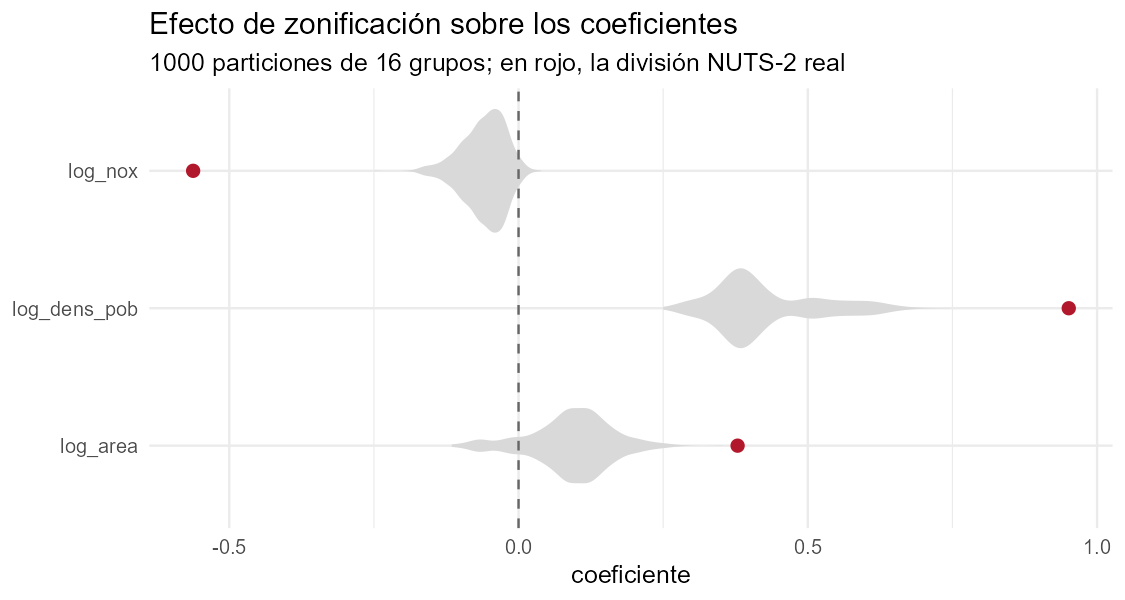
\includegraphics[width=0.70\textwidth]{43_maup_zonificacion.png}
\end{center}

Sobre \num{1000} particiones alternativas de igual tamaño el coeficiente
industrial se mueve en $[\num{-0.146},\num{0.003}]$ con mediana \num{-0.053}:
el valor observado sobre \textsc{nuts}-2 queda \emph{fuera del rango completo}
por un factor de casi cuatro. La densidad de población resulta significativa en
el \SI{100}{\percent} de las particiones; la industria, en el
\SI{2.5}{\percent}, por debajo del nivel nominal.

Notablemente, \textbf{Madrid nunca queda aislada} en ninguna de las mil
réplicas: el $k$-medias agrupa unas tres provincias por centro y Madrid está
rodeada en el centro de la meseta. La división \textsc{nuts}-2 la aísla por
razones históricas y políticas, no geométricas, y ese aislamiento es el
mecanismo del artefacto.

Los dos componentes se refuerzan: el de escala muestra que el efecto depende de
una sola observación, y el de zonificación, que ninguna partición alternativa
en dieciséis grupos la produce. No es que dieciséis unidades sean pocas: es que
\emph{esas} dieciséis aíslan Madrid.

\subsection*{Descomposición de varianza y cota del efecto}

La descomposición \textsc{lmg} del modelo de tres predictores asigna el
\SI{84.5}{\percent} del $R^2$ a la densidad de población, el
\SI{10.8}{\percent} al área y el \SI{4.9}{\percent} a las emisiones. Con el
conjunto completo de covariables, la varianza única total es solo el
\SI{19.7}{\percent} del $R^2$; el \SI{80.3}{\percent} restante es compartida
entre bloques y no atribuible a ningún mecanismo por separado. Este reparto es
en sí un resultado: a escala provincial los mecanismos son estadísticamente
inseparables.

El resultado más informativo del modelo areal \textbf{no es un $p$-valor sino
una cota}. El intervalo de confianza al \SI{95}{\percent} del coeficiente
industrial es $[\num{-0.1006},\num{0.0617}]$; recorriendo todo el rango
observado de emisiones, el efecto máximo compatible con los datos es
\SI{0.956}{\micro\gram\per\cubic\metre}, el \SI{22.3}{\percent} de la media
areal nacional (\SI{4.28}{\micro\gram\per\cubic\metre}). No es que ignoremos si
la industria influye: sabemos que \emph{no puede influir más que eso}.

% -----------------------------------------------------------------------------
\subsection*{Objetivo c): el patrón puntual industrial}

\rotulo{Figura 9}{Patrón industrial y contraste de cuadrantes}

\begin{center}
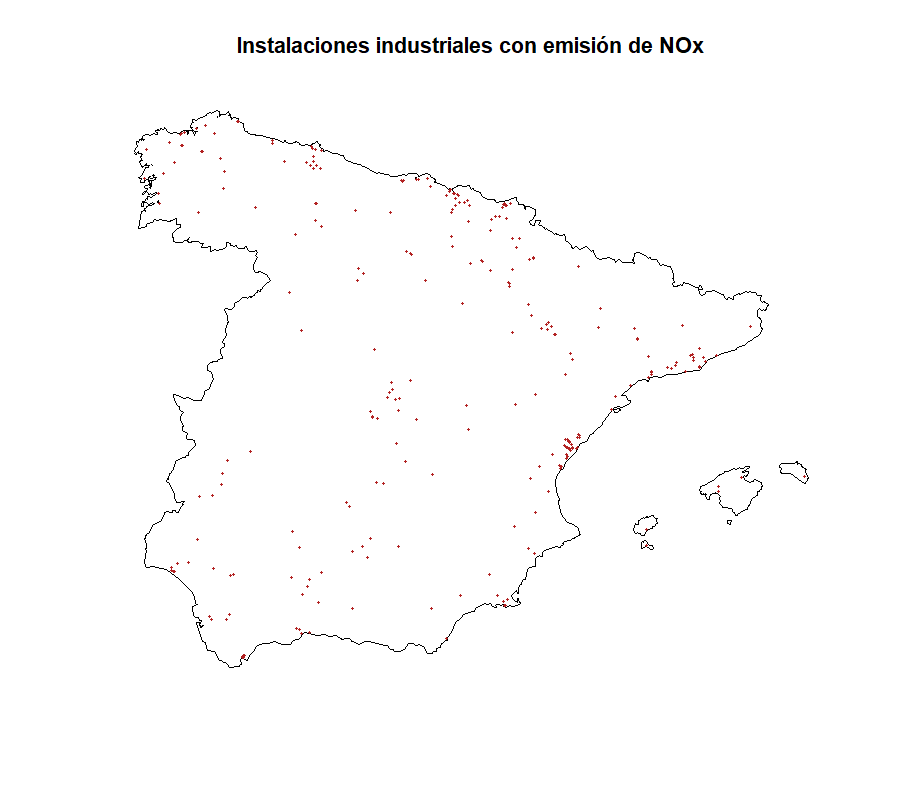
\includegraphics[width=0.48\textwidth]{20_patron_industrial.png}\hfill
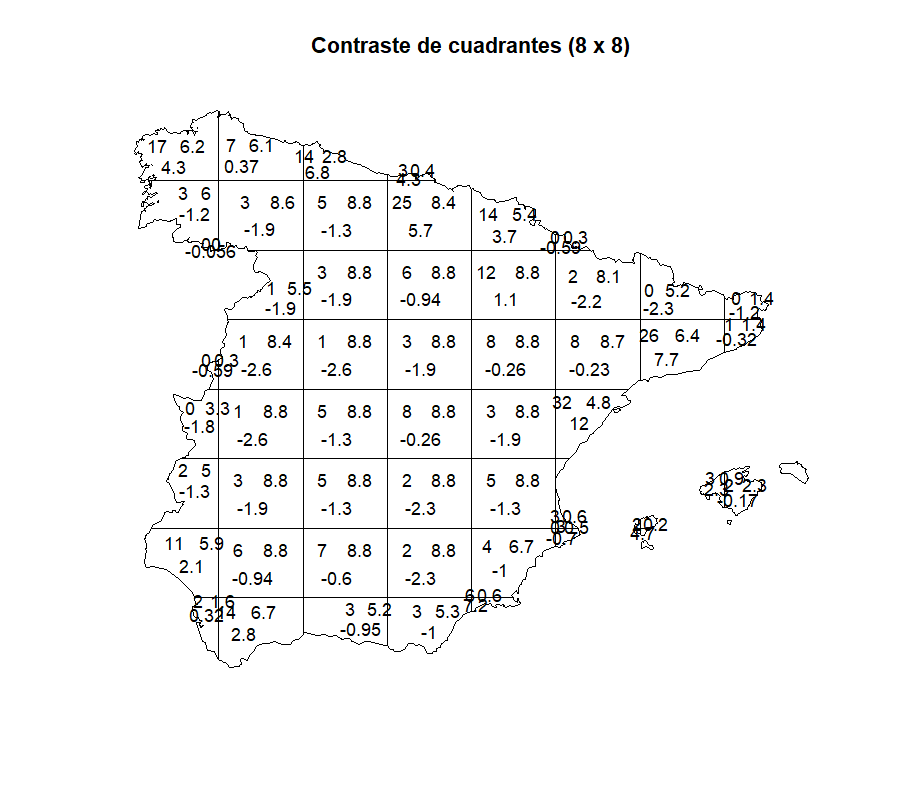
\includegraphics[width=0.48\textwidth]{22_cuadrantes.png}
\end{center}

El patrón consta de \num{297} instalaciones tras deduplicar por
\texttt{InspireSiteId} —de \num{103299} registros brutos—, sobre una ventana de
\SI{504327}{\kilo\metre\squared} (el dominio dilatado \SI{1}{\kilo\metre} para
no perder instalaciones portuarias, un \SI{1.2}{\percent} más que el dominio
nominal). La deduplicación no es limpieza de datos: es lo que hace que el
patrón cumpla la propiedad de proceso \textbf{ordenado}.

El contraste de cuadrantes por Monte Carlo con $m=\num{52}$ teselas rechaza la
aleatoriedad espacial completa:
$X^2=\sum_i (n_i-e_i)^2/e_i = \num{531.64}$, $p=\num{0.002}$. Este rechazo es
lo que obliga a que toda la caracterización posterior sea
\textbf{inhomogénea}: la $K$ estacionaria no es aplicable a un proceso cuya
homogeneidad acaba de rechazarse.

\rotulo{Figura 10}{Intensidad estimada del proceso puntual}

\begin{center}
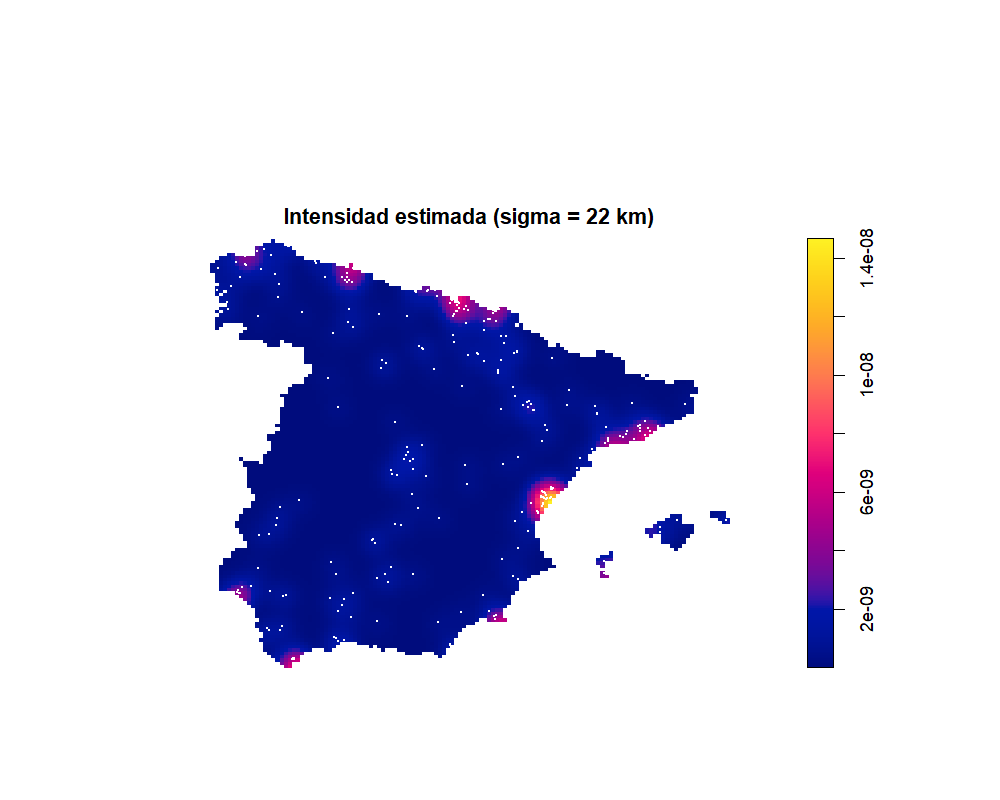
\includegraphics[width=0.60\textwidth]{21_intensidad.png}
\end{center}

\rotulo{Tabla 8}{Efectos multiplicativos sobre la intensidad, por rango
intercuartílico de cada covariable $Z_j(\loc)$}

\begin{center}
\small
\begin{tabular}{@{}lcc@{}}
\toprule
\textbf{Covariable} & \textbf{Factor} & \textbf{$p$} \\
\midrule
Suelo industrial & \num{3.94} & $<\num{0.001}$ \\
Superficie artificial & \num{1.32} & $<\num{0.001}$ \\
Transporte & \num{0.75} & $<\num{0.001}$ \\
\rowcolor{grisc}
Densidad de población & \num{0.999} & \num{0.997} \\
\bottomrule
\end{tabular}
\end{center}

El efecto del suelo industrial es de $\times\num{3.94}$ por rango
intercuartílico, mientras que \textbf{la densidad de población no es
significativa} ($\times\num{0.999}$, $p=\num{0.997}$). Este resultado merece
énfasis por dos motivos. El primero es sustantivo: condicionando en uso del
suelo, dónde vive la gente no predice dónde se instala la industria, lo que
constituye evidencia directa contra la hipótesis de colinealidad total entre
ambos mecanismos. El segundo es que \num{0.999} es esencialmente el valor de
referencia bajo independencia, $g_2=1$.

\rotulo{Figura 11}{Funciones de segundo orden: $K$ y $g$ inhomogéneas}

\begin{center}
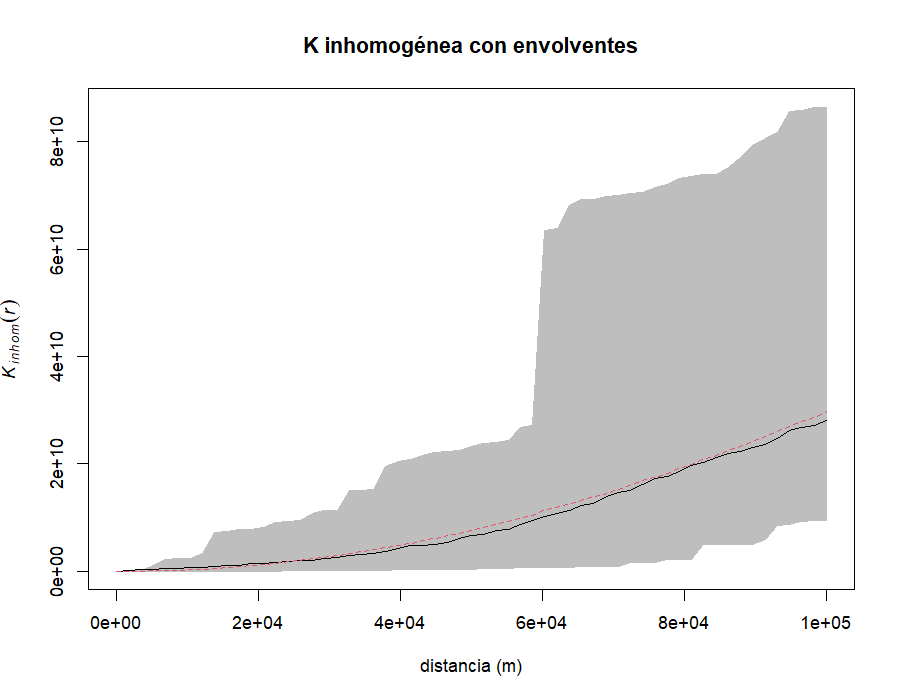
\includegraphics[width=0.48\textwidth]{23_Kinhom.png}\hfill
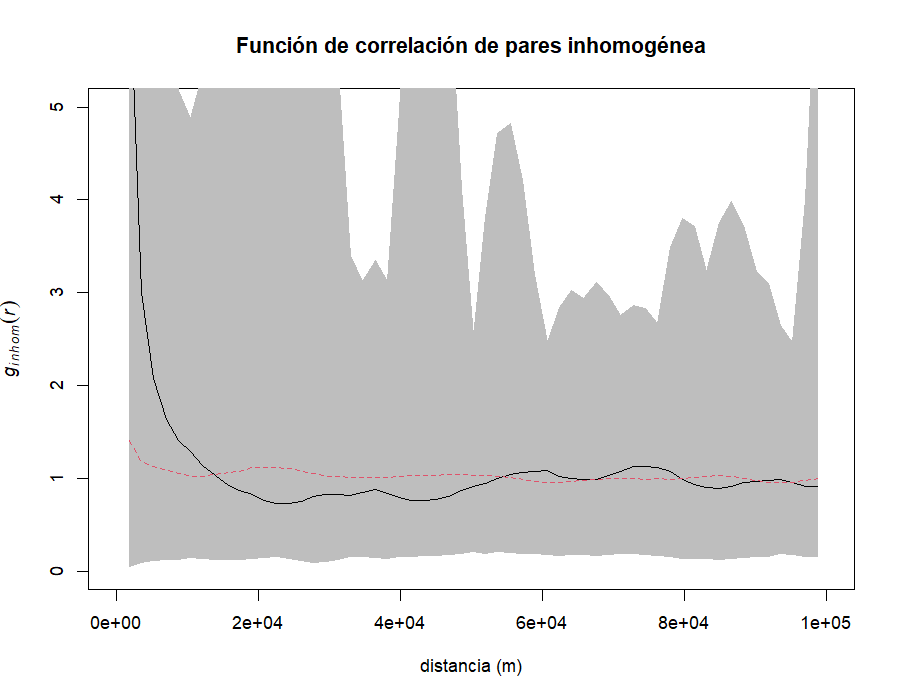
\includegraphics[width=0.48\textwidth]{24_ginhom.png}
\end{center}

Las curvas empíricas salen de las envolventes de Monte Carlo (\num{199}
simulaciones): hay agregación significativa frente a un proceso de Poisson
inhomogéneo con la misma intensidad. Bajo independencia, $g_2$ valdría
\num{1} y $K(t)$ sería $\pi t^2$; ambas se separan de su referencia.

\rotulo{Figura 12}{Residuos del modelo de intensidad y $K$ residual}

\begin{center}
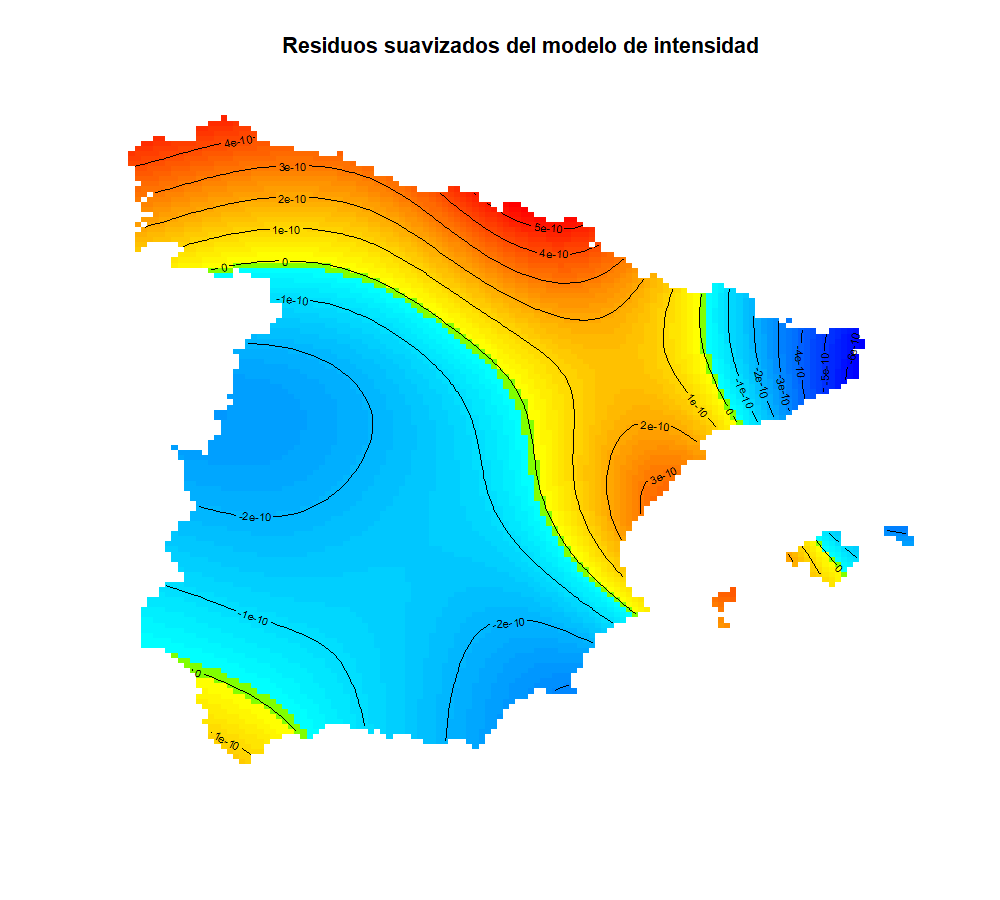
\includegraphics[width=0.48\textwidth]{25_residuos_ppm.png}\hfill
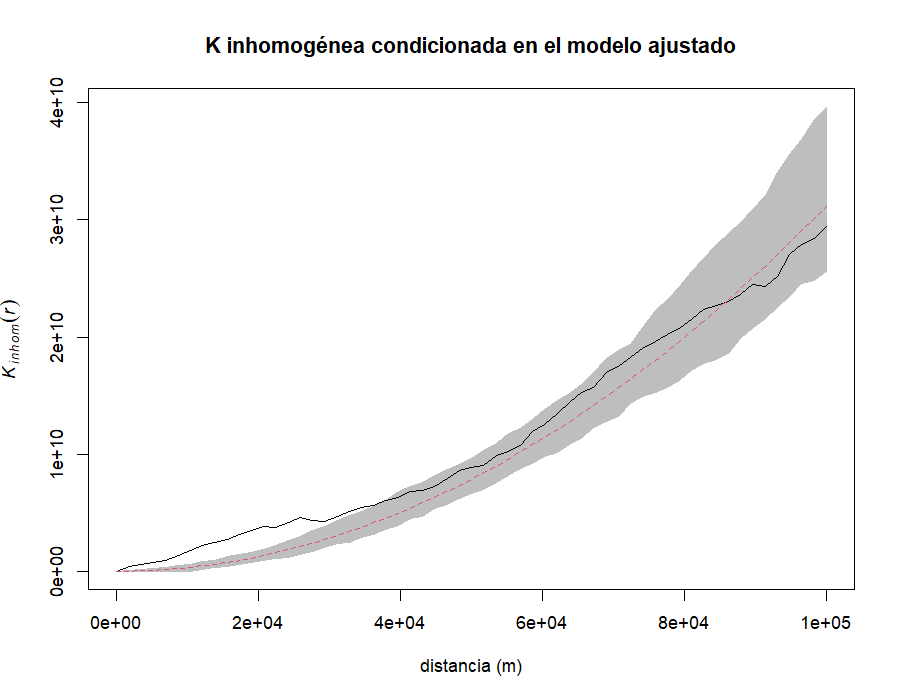
\includegraphics[width=0.48\textwidth]{26_Kinhom_residual.png}
\end{center}

Los residuos suavizados muestran zonas donde hay más instalaciones de las que
predicen las covariables. La $K$ inhomogénea sobre los residuos revela
\textbf{agregación no explicada hasta \SI{38}{\kilo\metre}}: queda estructura
que las covariables observadas no capturan, y es esa estructura la que motiva
pasar a un modelo de conglomerados.

El proceso agregado ajustado —padres no observados, descendencia con dispersión
gaussiana— estima $\sigma=\SI{2.7}{\kilo\metre}$, es decir un
\textbf{diámetro efectivo del distrito de \SI{10.7}{\kilo\metre}}, con
\num{520} conglomerados y probabilidad de hermandad $p_{sib}=\num{0.915}$.

\subsection*{El umbral de declaración sesga la intensidad, no la escala}

El registro E-PRTR solo recoge instalaciones que declaran más de
\SI{100}{\tonne} anuales de \ce{NOx} —la marca mínima observada es
\SI{102}{\tonne}—, de modo que el patrón observado $Y$ es un subconjunto del
patrón industrial real $Z$. Si cada evento se retiene de forma independiente
con probabilidad $p$, se tiene

\begin{equation}
\lambda_Y(\loc) = p\,\lambda_Z(\loc)
\qquad\text{pero}\qquad
K_Y(t) = K_Z(t).
\end{equation}

Es decir: el truncamiento sesga la intensidad a la baja por un factor $p$, pero
\textbf{deja invariante la función $K$}, y con ella la escala de agregación.
Como el resultado central depende de $K$ y no de $\lambda$, el umbral no toca
la magnitud que se estima. La salvedad que debe declararse es que el
adelgazamiento no sería independiente de la posición si las instalaciones
grandes se agruparan de forma distinta a las pequeñas; la correlación de marcas
es el diagnóstico de eso y no muestra tal patrón.

% -----------------------------------------------------------------------------
\subsection*{Objetivo d): convergencia de escalas}

\rotulo{Figura 13}{Superficie de presión de emisión y curva de escala}

\begin{center}
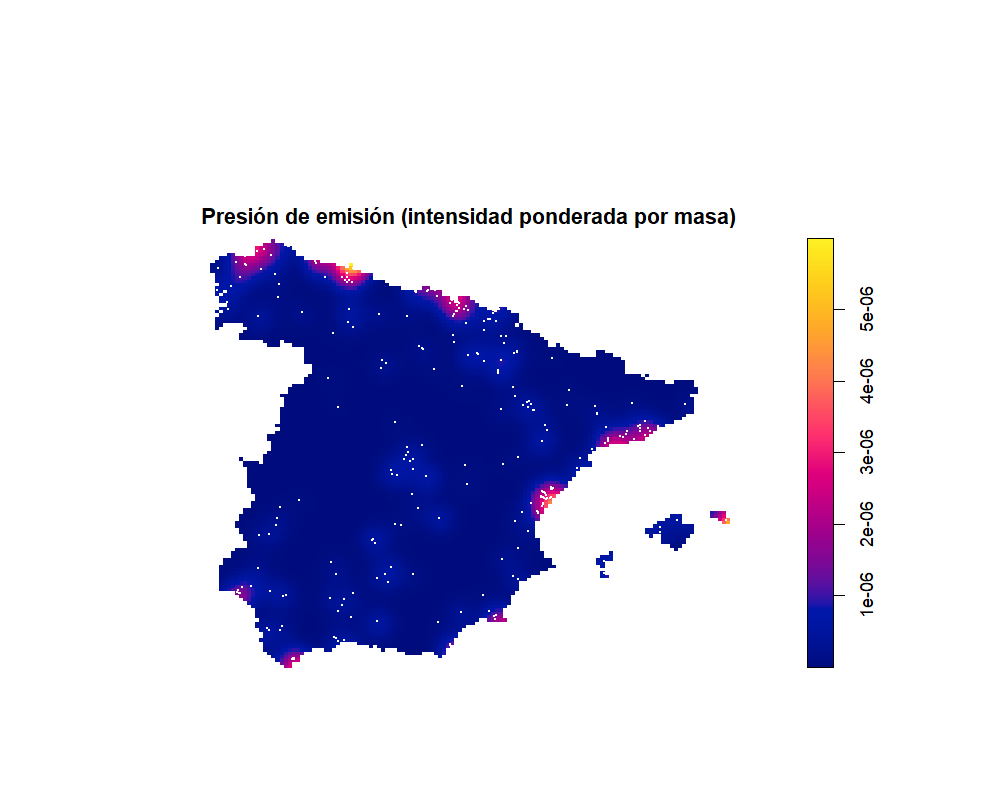
\includegraphics[width=0.48\textwidth]{28_presion_emision.png}\hfill
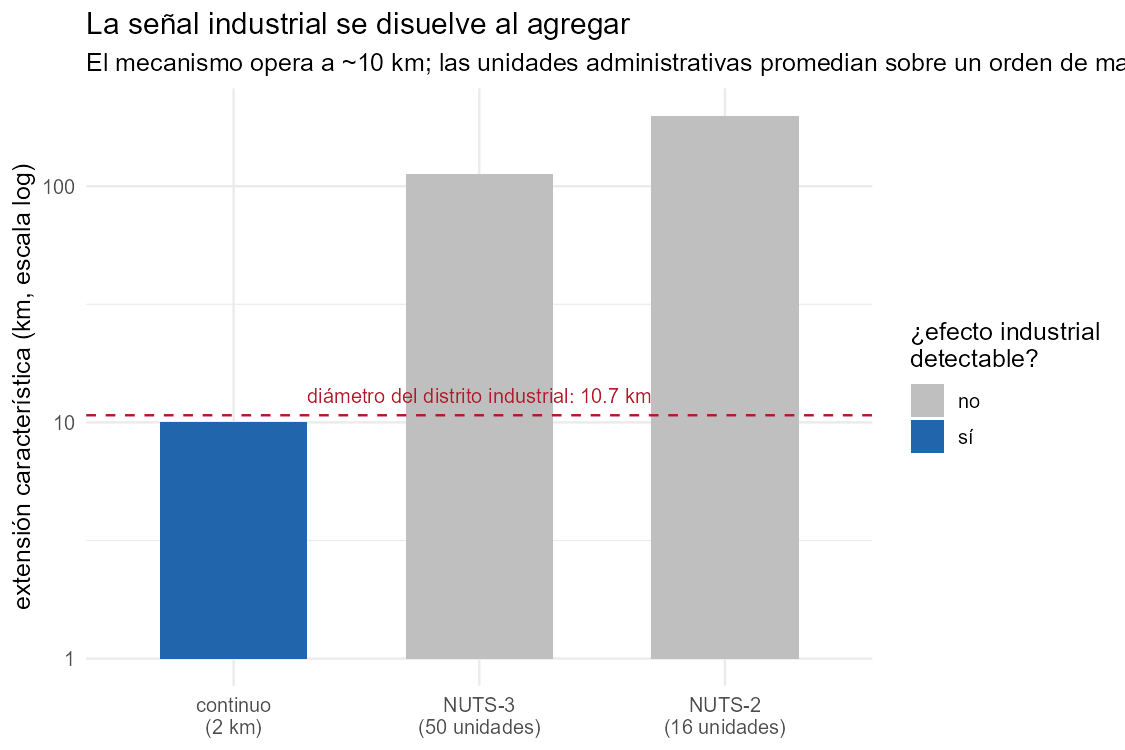
\includegraphics[width=0.48\textwidth]{50_curva_escala.png}
\end{center}

\rotulo{Tabla 9}{Barrido de anchos de banda $h$}

\begin{center}
\small
\begin{tabular}{@{}lcc@{}}
\toprule
\textbf{$h$ (\si{\kilo\metre})} & \textbf{RMSE} & \textbf{$\Delta$AIC} \\
\midrule
--- (base) & \num{3.6568} & \num{2.777} \\
5   & \num{3.6879} & \num{2.777} \\
\rowcolor{grisc}
10  & \num{3.6420} & \num{0.000} \\
15  & \num{3.6538} & \num{1.463} \\
25  & \num{3.6690} & \num{5.800} \\
40  & \num{3.6660} & \num{7.121} \\
60  & \num{3.6723} & \num{9.656} \\
100 & \num{3.6741} & \num{12.937} \\
\bottomrule
\end{tabular}
\end{center}

El barrido produce una curva en U limpia con mínimo en
$h=\SI{10}{\kilo\metre}$. El contraste $F$ frente al modelo sin presión
industrial da $F=\num{13.86}$, $p=\num{2.5e-4}$, y el $R^2$ ajustado pasa de
\num{0.754} a \num{0.769}. Multiplicar por $e$ la presión industrial eleva el
\ce{NO2} un \SI{6.35}{\percent}.

Se declara también lo que este resultado \emph{no} dice: la mejora del RMSE es
del \SI{0.41}{\percent}. El efecto es estadísticamente robusto pero de escaso
poder predictivo, algo coherente con la exclusión de Canarias del dominio.

\rotulo{Figura 14}{Escala de influencia estimada}

\begin{center}
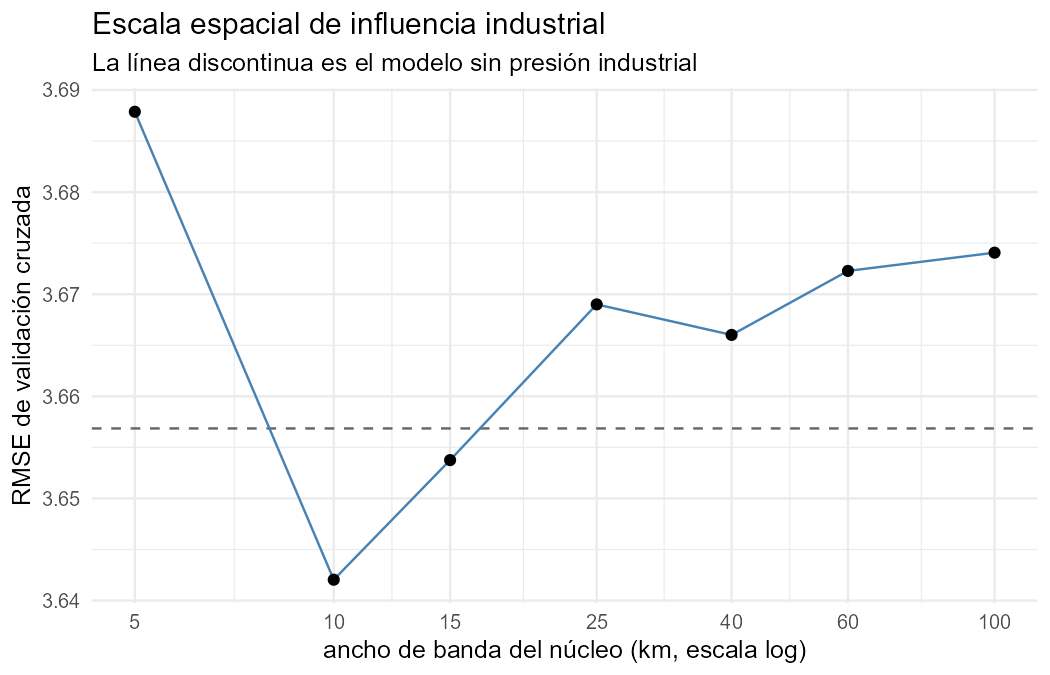
\includegraphics[width=0.62\textwidth]{30_escala_influencia.png}
\end{center}

\rotulo{Tabla 10}{Dos estimaciones independientes de la escala industrial}

\begin{center}
\small
\begin{tabular}{@{}llc@{}}
\toprule
\textbf{Magnitud} & \textbf{Datos usados} & \textbf{km} \\
\midrule
Diámetro del distrito (proceso agregado) & solo coordenadas & \num{10.7} \\
Escala de influencia (barrido de $h$) & coordenadas + concentraciones &
\num{10.0} \\
\midrule
\rowcolor{grisc}
\textbf{Razón} & & \textbf{\num{0.93}} \\
\bottomrule
\end{tabular}
\end{center}

Este es el hallazgo central. Las dos estimaciones difieren en un
\SI{7}{\percent} y \textbf{ninguna utiliza la información de la otra}: la
primera solo observa coordenadas de instalaciones y no mira ninguna
concentración; la segunda observa concentraciones y pregunta a qué distancia
deja de notarse la emisión. No existe razón aritmética para que coincidan.

La convergencia se verificó dos veces sobre patrones de puntos distintos. Antes
de una depuración del preprocesado que colapsó tres instalaciones duplicadas,
las cifras eran \SI{9.5}{} y \SI{10.0}{\kilo\metre} (razón \num{1.05});
después, \SI{10.7}{} y \SI{10.0}{\kilo\metre} (razón \num{0.93}). Que la
coincidencia sobreviva a un cambio no planeado en los datos de entrada es
evidencia de que no es un artefacto de un ajuste concreto.

\subsection*{Por qué el efecto desaparece al agregar}

\rotulo{Figura 15}{Las tres escalas espaciales sobre el mismo territorio}

\begin{center}
\includegraphics[width=\textwidth]{45_tres_escalas.png}
\end{center}

Los tres paneles comparten extensión y hacen visible el argumento central. Las
\num{16} comunidades autónomas promedian \SI{31158}{\kilo\metre\squared} cada
una; las \num{50} provincias, \SI{9970}{\kilo\metre\squared}. Los distritos
industriales del panel derecho —la unión de discos del diámetro estimado
(\SI{10.7}{\kilo\metre}) en torno a las \num{297} instalaciones, recortada al
dominio— forman \num{169} piezas conexas que suman
\SI{18076}{\kilo\metre\squared}, el \textbf{\SI{3.6}{\percent} del
territorio}.

Conviene precisar qué representa ese tercer panel: el proceso agregado estima
\num{520} centros latentes, pero \emph{sus posiciones no se observan}. Lo
dibujado es la huella espacial del mecanismo a la escala estimada, no los
padres del proceso. Los distritos aparecen rotulados por su instalación de
mayor emisión, ordenados por \ce{NOx} acumulado.

\rotulo{Figura 16}{Extensión característica de cada soporte espacial}

\begin{center}
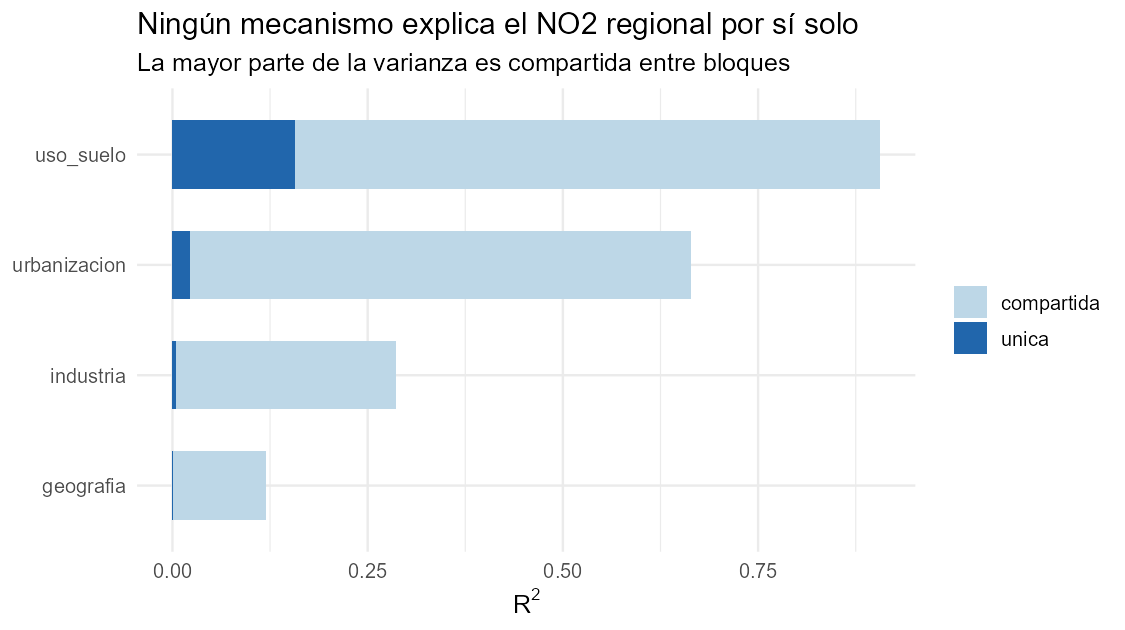
\includegraphics[width=0.62\textwidth]{51_sintesis_bloques.png}
\end{center}

La explicación es geométrica y cuantificable. La provincia media española mide
\SI{9970}{\kilo\metre\squared}, un disco equivalente de \SI{113}{\kilo\metre}
de diámetro. Un distrito de \SI{10}{\kilo\metre} de \textbf{diámetro} cubre el
\SI{0.8}{\percent} de esa superficie, y el conjunto de los \num{297} focos
—con solapamiento entre los próximos— ocupa el \SI{3.6}{\percent} del dominio.
Agregar a \textsc{nuts}-3 promedia la señal industrial contra \textbf{dos
órdenes de magnitud de territorio donde el mecanismo no opera}.

Las dos cifras son complementarias y conviene no confundirlas: el
\SI{0.8}{\percent} mide un distrito aislado frente a su provincia, y es lo que
explica por qué el efecto se diluye al agregar; el \SI{3.6}{\percent} mide el
agregado nacional, y acota cuánto territorio está expuesto al mecanismo.

La urbanización sobrevive a la agregación porque \emph{opera} a escala
provincial; la industria no. La diferencia no está en la intensidad del
mecanismo sino en su alcance espacial.

\subsection*{Implicaciones para la gestión}

\rotulo{Figura 17}{Exposición poblacional}

\begin{center}
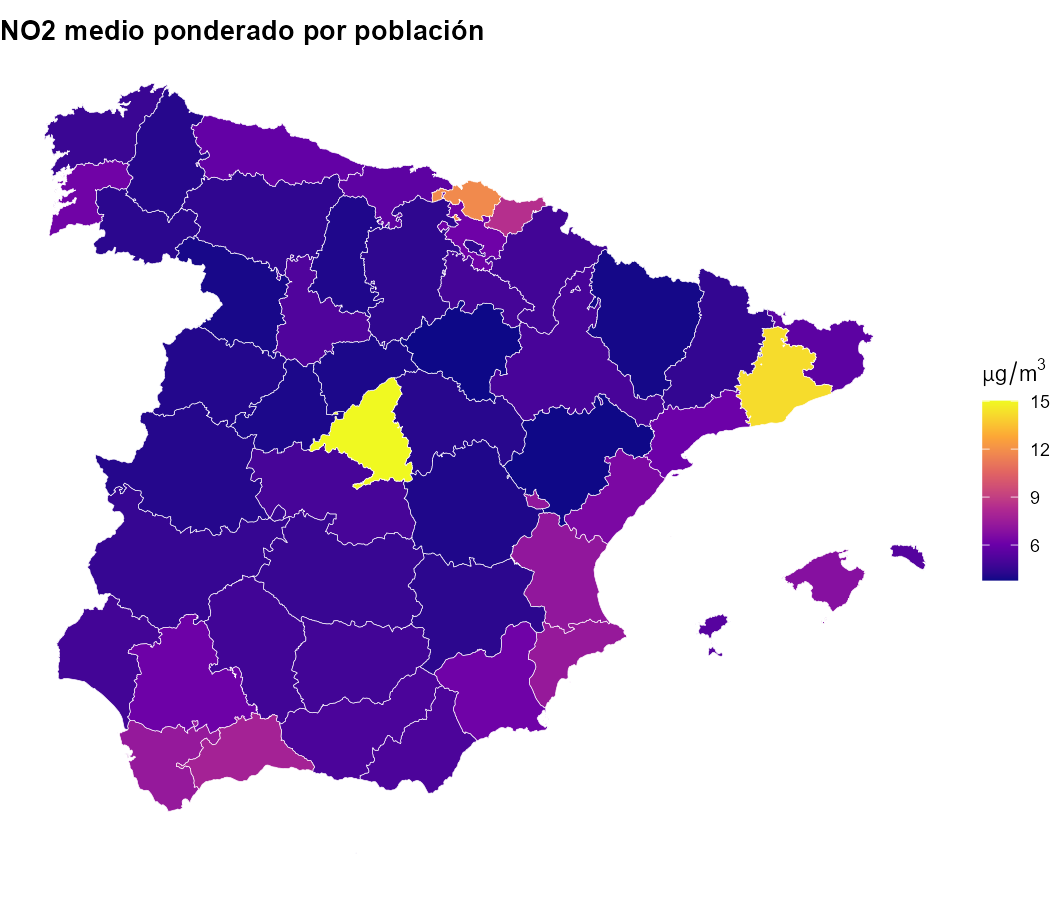
\includegraphics[width=0.48\textwidth]{13_exposicion_poblacional.png}\hfill
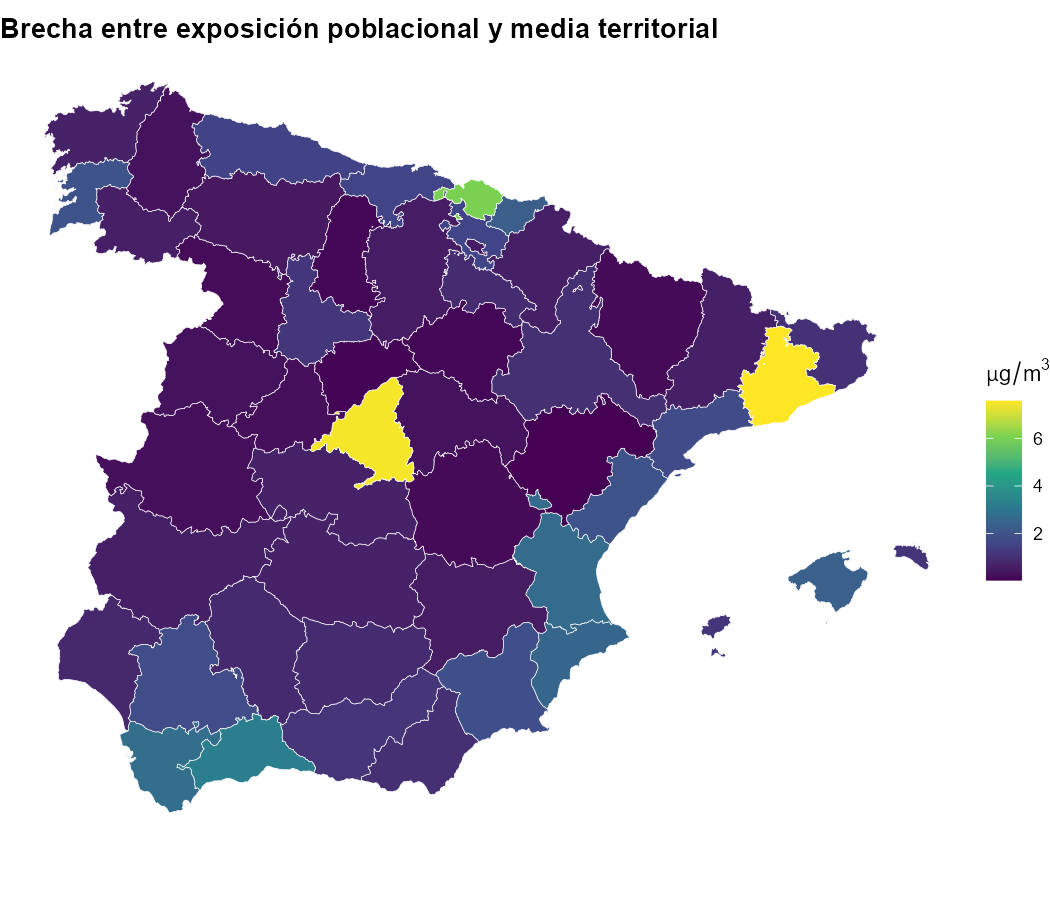
\includegraphics[width=0.48\textwidth]{15_brecha_exposicion.png}
\end{center}

La ponderación dasimétrica por población eleva la exposición estimada de Madrid
de \SI{7.52}{} a \SI{15.01}{\micro\gram\per\cubic\metre} y la de Barcelona de
\SI{6.64}{} a \SI{14.21}{\micro\gram\per\cubic\metre}. Tres provincias superan
el \SI{10}{\percent} de población por encima de
\SI{20}{\micro\gram\per\cubic\metre}: Madrid (\SI{37.3}{\percent}), Barcelona
(\SI{30.6}{\percent}) y Bizkaia (\SI{22.7}{\percent}).

El contraste que cierra el análisis: el \SI{43.3}{\percent} de las estaciones
de tráfico superan hoy los \SI{20}{\micro\gram\per\cubic\metre}, frente al
\SI{0.16}{\percent} de la superficie de fondo. España cumple con holgura la
directiva vigente y tiene margen frente al umbral de 2030, pero está lejos de
la recomendación de la OMS, y el problema reside en una escala por debajo de la
que este trabajo puede resolver.

% =============================================================================
\section{Discusión y limitaciones}

\subsection*{Qué aporta cada rama}

Ninguna de las tres ramas responde la pregunta por sí sola.

La \textbf{variación continua} proporciona concentración en puntos no
muestreados con incertidumbre propagada, y separa campo de fondo de recargo
microescala; el modelo areal no puede recuperar el interior de la unidad y el
proceso puntual no observa concentraciones.

El \textbf{proceso puntual} establece dónde se ubican las fuentes y por qué, y
detecta distritos tras condicionar en covariables; la rama continua trata las
fuentes como covariable dada, y la areal no distingue veinte instalaciones
agrupadas de veinte dispersas.

La \textbf{variación discreta} produce cifras sobre la unidad en que se legisla
y pondera por población, y es la única que entrega una cota utilizable en
gestión.

Y la comparación entre escalas exige dos ramas metodológicamente
independientes: es el único resultado que ninguna produce sola.

\subsection*{Limitaciones, en orden de importancia}

\begin{enumerate}[label=(\roman*), leftmargin=1.8em, itemsep=2pt]
  \item El umbral de declaración E-PRTR es de \SI{100}{\tonne} anuales; el
  patrón representa grandes emisores. Como se demostró, sesga $\lambda$ pero no
  $K$: la escala estimada sobrevive al truncamiento.
  \item Canarias, con el \SI{24}{\percent} del \ce{NOx} industrial español,
  queda fuera del dominio. Las conclusiones aplican a la España peninsular y
  balear.
  \item La superficie modela \ce{NO2} de fondo, no exposición máxima. Los picos
  de tráfico ocurren por debajo de la resolución de \SI{2}{\kilo\metre}: el
  análisis señala su propio punto ciego.
  \item La clase 121 de CORINE mezcla industria con comercio y logística, por
  lo que está casi colineal con urbanización. La señal industrial limpia es el
  patrón E-PRTR, no la cobertura del suelo.
  \item Con $n=\num{50}$ unidades areales el modelo tiene poca potencia; el
  diagnóstico de influyentes lo confirma. La cota del efecto industrial debe
  leerse teniendo esto presente.
  \item Las envolventes de Monte Carlo se calculan con $\lambda$ estimada de
  los propios datos, lo que hace el contraste ligeramente anticonservador.
  \item El modelo de correlación seleccionado corresponde al límite suave de la
  familia de Matérn e implica variación por debajo de la menor distancia entre
  estaciones.
  \item La cobertura empírica al \SI{95}{\percent} es \num{0.910}, por debajo
  de la nominal.
\end{enumerate}

\subsection*{Trabajo futuro}

Una formulación jerárquica bayesiana con \textsc{spde} (Lindgren et al., 2011)
permitiría propagar la incertidumbre de la superficie predicha hacia el modelo
areal en lugar de tratarla como dato. Esta vía es además la que unifica las
ramas: el enfoque \textsc{spde} representa un proceso gaussiano continuo como
un campo markoviano gaussiano, es decir, aproxima $\varesp\Rphi$ por una
precisión $\Prec$ dispersa. Y un proceso agregado es un Poisson doblemente
estocástico: si $\log\Lambda(\loc)$ fuera el mismo campo gaussiano que modela
el fondo, las ramas continua y puntual quedarían formuladas en un único modelo.
La extensión temporal a la serie 2019--2023 permitiría explotar el cierre de
instalaciones como cuasiexperimento.

% =============================================================================
\section{Conclusiones}

\begin{enumerate}[leftmargin=1.6em, itemsep=4pt]
  \item \textbf{Convergencia de escalas.} Dos estimaciones metodológicamente
  independientes —una que solo observa coordenadas de instalaciones, otra que
  observa concentraciones— sitúan la escala de la influencia industrial sobre
  el \ce{NO2} de fondo en España en torno a \SI{10}{\kilo\metre}, con una razón
  entre ambas de \num{0.93}. \textbf{La unidad de influencia es el distrito
  industrial, no la instalación aislada.}

  \item \textbf{Variación continua.} El campo de fondo tiene un rango práctico
  de \SI{71}{\kilo\metre} que cae a \SI{24}{\kilo\metre} tras retirar la
  deriva: las covariables absorben el \SI{76}{\percent} de la varianza. La
  pepita del \SI{9.6}{\percent} indica que el \SI{90.4}{\percent} de la
  variabilidad está espacialmente estructurada, y el kriging con deriva externa
  reduce el error un \SI{34.3}{\percent} respecto al ordinario.

  \item \textbf{Variación discreta y \textsc{maup}.} El efecto industrial es
  indetectable a escala provincial, y la desaparición no obedece a falta de
  potencia sino a que la unidad de análisis promedia la señal sobre un
  territorio dos órdenes de magnitud mayor que su alcance. El resultado resiste
  cuatro intentos de refutación y \num{1000} zonificaciones alternativas. Se
  documentan los \emph{dos} componentes del \textsc{maup}, no solo el de
  escala, y se entrega una cota de
  \SI{0.956}{\micro\gram\per\cubic\metre} en lugar de un $p$-valor.

  \item \textbf{Procesos puntuales.} El patrón industrial rechaza la
  aleatoriedad espacial completa y presenta agregación no explicada hasta
  \SI{38}{\kilo\metre} tras condicionar en covariables de uso del suelo. La
  densidad de población no predice la localización industrial
  ($\times\num{0.999}$, $p=\num{0.997}$), lo que confirma que en España ambos
  mecanismos no son colineales.

  \item \textbf{Aportación metodológica.} El problema de la unidad de área
  modificable puede pasar de advertencia genérica a diagnóstico cuantitativo
  cuando se dispone de una escala de referencia estimada externamente.
  \textbf{Sin la rama de procesos puntuales, el resultado nulo areal sería
  indistinguible de una ausencia real de efecto.}
\end{enumerate}

% =============================================================================
\section{Disponibilidad y reproducibilidad}

El código completo, los guiones de descarga y las instrucciones de ejecución
están disponibles en \url{https://github.com/randyfernandezp/no2-espana}. El
repositorio incluye un guion de verificación de integridad
(\texttt{R/99\_verificar.R}) que comprueba invariantes de conservación y
frescura de los ficheros derivados.

Cada cifra de este trabajo procede de un guion ejecutable. En particular, la
tabla~7 y el diagnóstico de influyentes de la sección de escala se regeneran
con \texttt{R/47\_nuts2\_especificacion.R}, que además valida la convención de
agregación comparando las tres alternativas contra la respuesta almacenada por
el pipeline; y la figura~15 con \texttt{R/46\_tres\_escalas.R}. Ninguna cifra
del texto se ha transcrito a mano desde una sesión interactiva.

% =============================================================================
\section{Referencias bibliográficas}

\begin{small}
\begin{list}{}{\leftmargin=1.4em \itemindent=-1.4em \itemsep=2pt}
\item Anselin, L. (1988). \emph{Spatial Econometrics: Methods and Models}.
Springer, Dordrecht.
\item Anselin, L., Bera, A. K., Florax, R., y Yoon, M. J. (1996). Simple
diagnostic tests for spatial dependence. \emph{Regional Science and Urban
Economics}, 26(1):77--104.
\item Baddeley, A., Rubak, E., y Turner, R. (2015). \emph{Spatial Point
Patterns: Methodology and Applications with R}. Chapman and Hall/CRC, Nueva
York.
\item Baddeley, A. J., Møller, J., y Waagepetersen, R. (2001). Non- and
semi-parametric estimation of interaction in inhomogeneous point patterns.
\emph{Statistica Neerlandica}, 54(3):329--350.
\item Banerjee, S., Carlin, B. P., y Gelfand, A. E. (2014). \emph{Hierarchical
Modeling and Analysis for Spatial Data}, 2.\textsuperscript{a} ed. Chapman and
Hall/CRC, Nueva York.
\item Beelen, R., Hoek, G., Vienneau, D., Eeftens, M., et al. (2013).
Development of \ce{NO2} and \ce{NOx} land use regression models for estimating
air pollution exposure in 36 study areas in Europe: The ESCAPE project.
\emph{Atmospheric Environment}, 72:10--23.
\item Bivand, R. y Piras, G. (2015). Comparing implementations of estimation
methods for spatial econometrics. \emph{Journal of Statistical Software},
63(18):1--36.
\item Chen, J., de Hoogh, K., Gulliver, J., Hoffmann, B., et al. (2019). A
comparison of linear regression, regularization, and machine learning
algorithms to develop Europe-wide spatial models of fine particles and nitrogen
dioxide. \emph{Environment International}, 130:104934.
\item Cressie, N. A. C. (1993). \emph{Statistics for Spatial Data}, ed.
revisada. Wiley, Nueva York.
\item Diggle, P. J. (2013). \emph{Statistical Analysis of Spatial and
Spatio-Temporal Point Patterns}, 3.\textsuperscript{a} ed. CRC Press.
\item Gelfand, A. E., Zhu, L., y Carlin, B. P. (2001). On the change of support
problem for spatio-temporal data. \emph{Biostatistics}, 2(1):31--45.
\item Gotway, C. A. y Young, L. J. (2002). Combining incompatible spatial data.
\emph{Journal of the American Statistical Association}, 97(458):632--648.
\item Grömping, U. (2006). Relative importance for linear regression in R: the
package relaimpo. \emph{Journal of Statistical Software}, 17(1):1--27.
\item Lee, D., Robertson, C., Ramsay, C., y Pyper, K. (2020). Quantifying the
impact of the modifiable areal unit problem when estimating the health effects
of air pollution. \emph{Environmetrics}, 31(8):e2643.
\item Lindgren, F., Rue, H., y Lindström, J. (2011). An explicit link between
Gaussian fields and Gaussian Markov random fields: the stochastic partial
differential equation approach. \emph{JRSS: Series B}, 73(4):423--498.
\item Moran, P. A. P. (1950). Notes on continuous stochastic phenomena.
\emph{Biometrika}, 37(1/2):17--23.
\item Openshaw, S. y Taylor, P. J. (1979). A million or so correlation
coefficients: three experiments on the modifiable areal unit problem. En
Wrigley, N. (ed.), \emph{Statistical Applications in the Spatial Sciences},
pp. 127--144. Pion, Londres.
\item Parenteau, M.-P. y Sawada, M. C. (2011). The modifiable areal unit
problem (MAUP) in the relationship between exposure to \ce{NO2} and respiratory
health. \emph{International Journal of Health Geographics}, 10:58.
\item Pebesma, E. J. (2004). Multivariable geostatistics in S: the gstat
package. \emph{Computers \& Geosciences}, 30(7):683--691.
\item Veefkind, J. P., Aben, I., McMullan, K., et al. (2012). TROPOMI on the
ESA Sentinel-5 Precursor. \emph{Remote Sensing of Environment}, 120:70--83.
\item World Health Organization (2021). \emph{WHO global air quality
guidelines}. ISBN 978-92-4-003422-8.
\end{list}
\end{small}

\end{document}
